%%%%%%%%%%%%%%%%%%%%%%%%%%%%%%%%%%%%%%%%%
% Focus Beamer Presentation
% LaTeX Template
% Version 1.0 (8/8/18)
%
% This template has been downloaded from:
% http://www.LaTeXTemplates.com
%
% Original author:
% Pasquale Africa (https://github.com/elauksap/focus-beamertheme) with modifications by 
% Vel (vel@LaTeXTemplates.com)
%
% Template license:
% GNU GPL v3.0 License
%
% Important note:
% The bibliography/references need to be compiled with bibtex.
%
%%%%%%%%%%%%%%%%%%%%%%%%%%%%%%%%%%%%%%%%%

%----------------------------------------------------------------------------------------
%	PACKAGES AND OTHER DOCUMENT CONFIGURATIONS
%----------------------------------------------------------------------------------------

\documentclass{beamer}

\usetheme{focus} % Use the Focus theme supplied with the template
% Add option [numbering=none] to disable the footer progress bar
% Add option [numbering=fullbar] to show the footer progress bar as always full with a slide count

% Uncomment to enable the ice-blue theme
%\definecolor{main}{RGB}{92, 138, 168}
%\definecolor{background}{RGB}{240, 247, 255}

%------------------------------------------------

\usepackage{booktabs} % Required for better table rules
\usepackage{gensymb}
%----------------------------------------------------------------------------------------
%	 TITLE SLIDE
%----------------------------------------------------------------------------------------

\title{GCIV2036-2 :\\ Convergence-confinement}

\subtitle{Présentation des résultats}

\author{Arthur Fanara \\ Bérengère Franck}

\titlegraphic{
\includegraphics[width=4cm]{Logo.jpg}} % Optional title page image, comment this line to remove it

\institute{ULiège \\ Professeur : F. Collin\\ Assistant : G. Corman}

\date{\today}

%------------------------------------------------

\begin{document}
\scriptsize
%------------------------------------------------

\begin{frame}
	\maketitle % Automatically created using the information in the commands above
\end{frame}

%----------------------------------------------------------------------------------------
%	 SECTION 1
%----------------------------------------------------------------------------------------

\begin{frame}{Sommaire}
  \tableofcontents
  % possibilité d'ajouter l'option [pausesections]
\end{frame}








\section{Introduction}


\begin{frame}{Introduction}

\begin{figure}
\centering
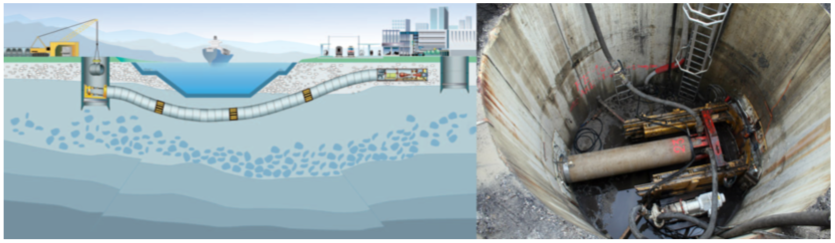
\includegraphics[width=10cm]{image.png}
\caption{Fonçage et puis d'accès}
\end{figure}

\begin{figure}
\centering
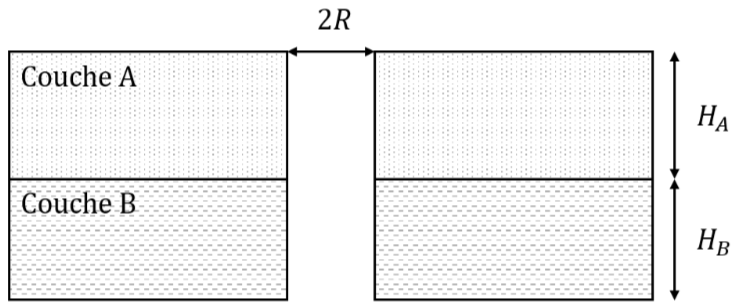
\includegraphics[width=6cm]{coupe.png}
\caption{Coupe verticale simplifiée du massif au niveau du puits}
\end{figure}

    
\end{frame}

\subsection{Présentation de la méthode}
\begin{frame}{Présentation de la méthode}
\begin{columns}

\begin{column}{0.54\textwidth}
  \begin{itemize}
      \item Le déconfinement du massif s'accompagne d'un déplacement des points situés à l'intrados : 
      $$f_m (\sigma , u) = 0$$
      
      \item Le comportement mécanique du soutènement est décrit par la relation 
      $$f_s (\sigma , u) = 0$$
      
      \item La méthode de convergence-confinement décrit la relation entre le massif et le soutènement et l'équilibre est donné par l'intersection des courbe de convergence et de confinement, c'est-à-dire par la solution du système constitué des deux équations précédentes. 
  \end{itemize}  
\end{column}


\begin{column}{0.45\textwidth}
\begin{figure}
\centering
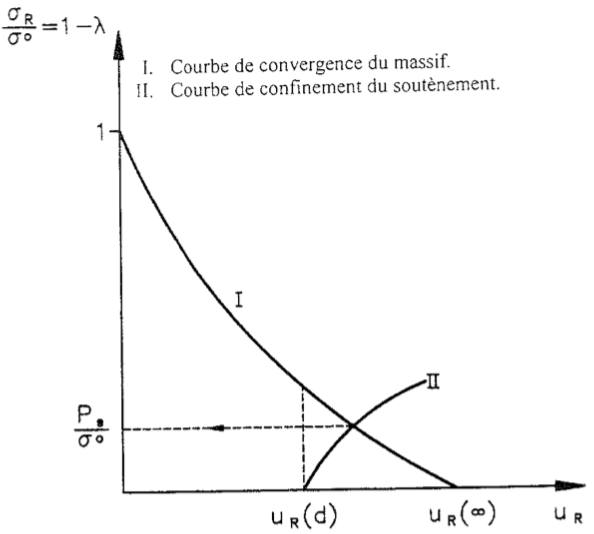
\includegraphics[width=5cm]{principe.png}
\end{figure}
\end{column}
\end{columns}

\end{frame}

\begin{frame}{Présentation de la méthode}

\begin{itemize}
    \item Le moment auquel le soutènement est installé est important 
    \item La méthode permet d'étudier le problème en 1D  (simplification par rapport à une étude 3D)
\end{itemize}
\vspace{0.3cm}

\underline{Hypothèses de la méthode}

  \begin{itemize}
    \item[$\bullet$] Matériau homogène et isotrope
    \item[$\bullet$] Champ de contraintes uniforme
    \item[$\bullet$] Conditions de symétrie de révolution
    \item[$\bullet$] Déformations planes dans le plan perpendiculaire à l'axe du puits
    \item[$\bullet$] Pas de variation de contraintes initiales 
  \end{itemize}   


\end{frame}



\subsection{Présentation du problème}
\begin{frame}{Présentation du problème}

\begin{columns}

\begin{column}{0.5\textwidth}


\underline{But :} tracer
\begin{itemize}
    \item le déplacement du massif $u_R$
    \item la distribution des contraintes $\sigma_r$ et $\sigma_{\theta}$ 
    \item les chemins de contraintes p-q et $\sigma_r - \sigma_{\theta}$
    \item les courbes caractéristiques du massif et du soutènement \newline
\end{itemize}

\underline{Données}

\begin{table}
    \centering
\begin{tabular}{|c|c|c|}
\hline
Données  & Valeur   & Unité   \\
\hline
$E_b$ & 30  & GPa   \\
\hline
$\nu_b$   & 0,2   & -   \\
\hline
\end{tabular}
\end{table}



\end{column}


\begin{column}{0.49\textwidth}

\begin{table}
    \centering
\begin{tabular}{|c|c|c|}
\hline
Données  & Valeur   & Unité   \\
\hline
$\gamma_{sat,sol}$    & 18   & $kN/m^3$   \\
\hline
$H_s$    & 7   & m   \\ 
\hline
 $H_A$   & 20   & m   \\ 
\hline
$H_B$    & 30   & m   \\ 
\hline
$E_A$    & 150   & MPa   \\ 
\hline
$E_B$    & 800   & MPa   \\ 
\hline
$\nu_A$    & 0,21   & -   \\ 
\hline
$\nu_B$    & 0,26   & -   \\ 
\hline
$c_A$    & \textbf{10}   & kPa   \\ 
\hline
$c_B$    & 100   & kPa  \\ 
\hline
$\phi_A$    & 22   & $\degree$   \\ 
\hline
$\phi_B$    & 27   & $\degree$   \\ 
\hline
$\psi_A$    & 3   & $\degree$   \\ 
\hline
$\psi_B$    & 4   & $\degree$   \\ 
\hline
$\gamma_{sat,A}$    & 23,5   & $kN/m^3$   \\
\hline
$\gamma_{sat,B}$    & 24   & $kN/m^3$   \\
\hline
$K_{0A}$    & 0,8   & -   \\ 
\hline
$K_{0B}$    & 1,05   & -   \\ 
\hline
\end{tabular}
\end{table}

\end{column}

\end{columns}
    
\end{frame}

\begin{frame}{Calcul des contraintes initiales}
Calcul de $\sigma_0$ pour chaque couche :\\
    
    \begin{itemize}
        \item[$\bullet$]$\sigma_{0A} = (\gamma_{sol} \cdot h_{sol} + \gamma_A \cdot h_A) \cdot K_{0A} = 476,8 \ kPa$ \\
    \item[$\bullet$]$ \sigma_{0B} = (\gamma_{sol} \cdot h_{sol} + \gamma_A \cdot h_A + \gamma_B \cdot h_B) \cdot K_{0B} = 1381,8 \ kPa$ \newline
    \end{itemize}


    
\end{frame}











\section{Étude élastique}

\subsection{Déplacement du massif}

\begin{frame}{Déplacement du massif}
    
\[\text{\textbf{Déplacement radial} :}\quad u_r (r)= \lambda \dfrac{R^2}{r} \dfrac{\sigma_0}{2G}\quad\text{où}\;r\in[R;3R]\;\text{et}\; \lambda\in[0;1]\]

\begin{figure}
    \centering
    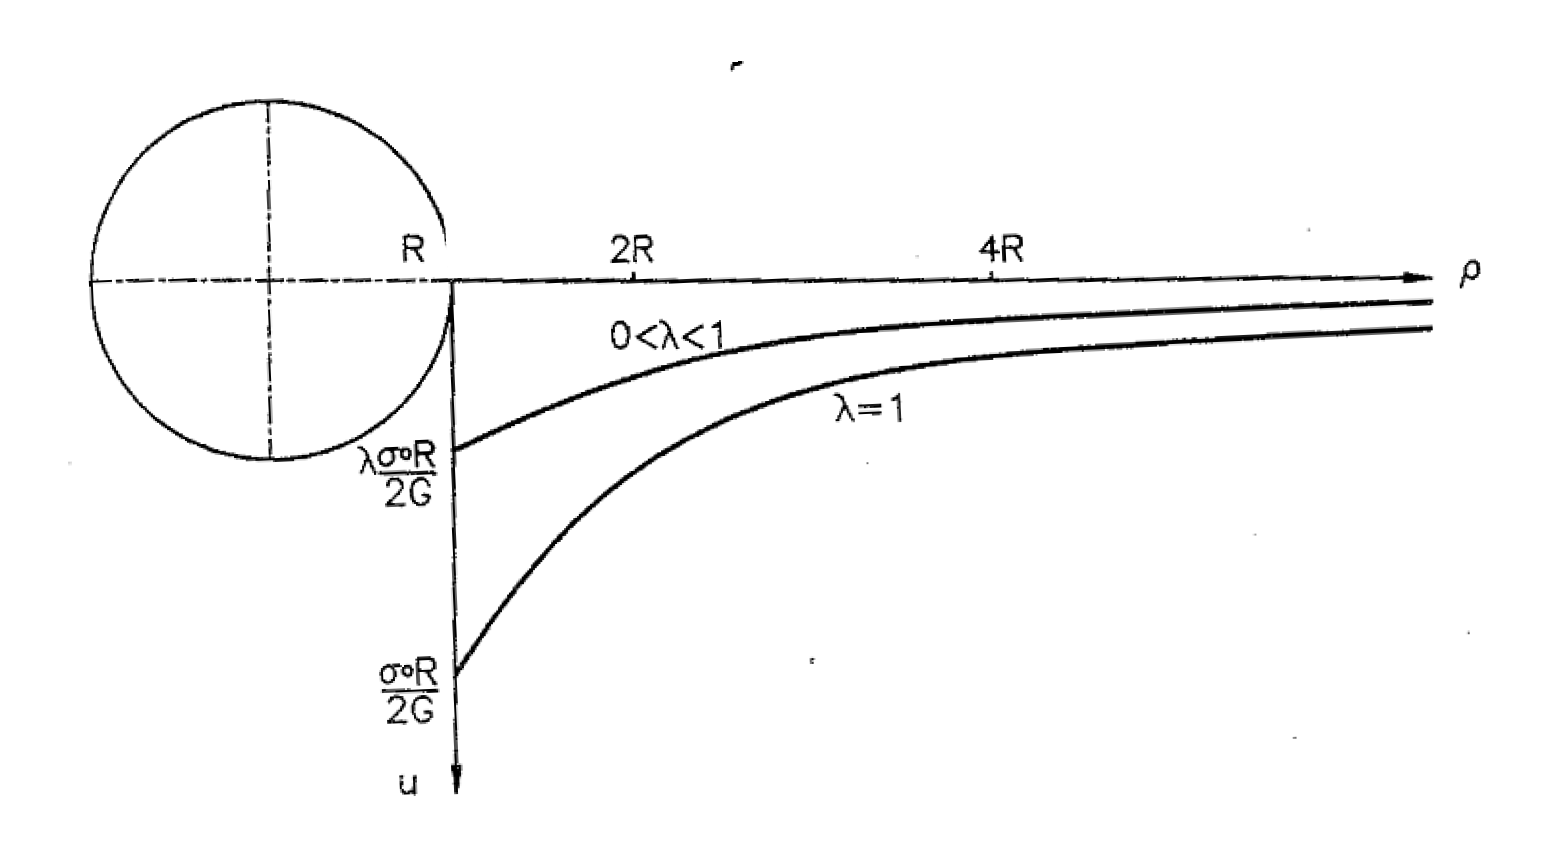
\includegraphics[height=4cm]{Results_ur.png}
    \caption{\scriptsize{Solution théorique de la relation $u(r)$}}
    \label{Results_ur}
\end{figure}

Première composante de la courbe caractéristique du massif : \[u_r(r=R) = \lambda \dfrac{\sigma_0 R}{2G}\]

%En principe, lorsque $x< 0,2R$ (près du front de taille), $\lambda$ dépend fortement du coefficient de poisson. Dans ce cas, on suppose un coefficient de poisson $\nu$ constant. (Pas étudié ici si?)

\end{frame}


\begin{frame}{Déplacement du massif}
    
    \begin{columns}
    \begin{column}{0.5\textwidth}
\begin{figure}
\centering
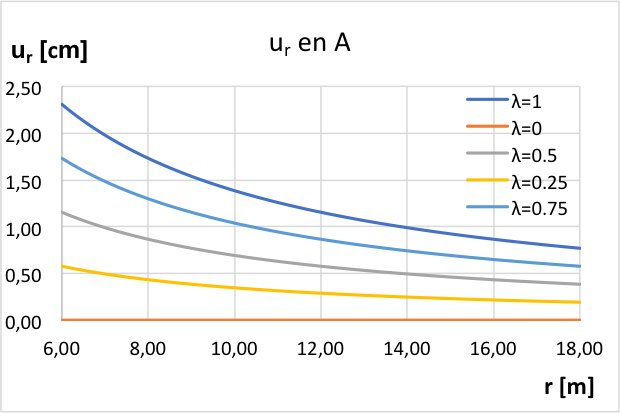
\includegraphics[width=5.5cm]{ur_A.png}
%\caption{Déplacement du massif en A}
\end{figure}
    \end{column}
    
    \begin{column}{0.5\textwidth}
\begin{figure}
\centering
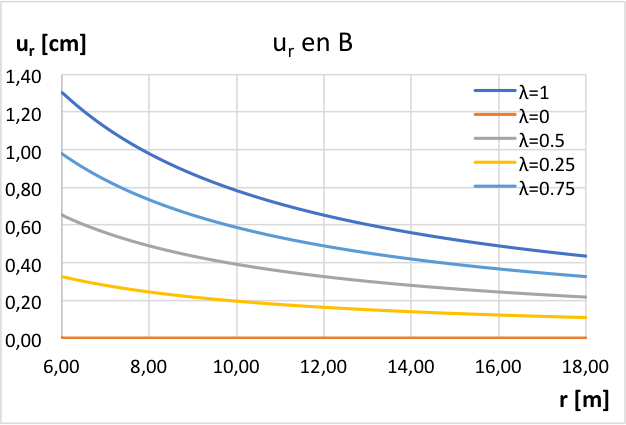
\includegraphics[width=5.5cm]{ur_B.png}
%\caption{Déplacement du massif en B}
\end{figure}
    \end{column}
    \end{columns}
    
\begin{itemize}
    \item Plus $\lambda$ est grand, plus le déplacement est grand
    
    \item Plusieurs valeurs de $\lambda$ : effet du déconfinement dans chaque couche\\ $\rightarrow$ la couche A est moins rigide
\end{itemize}
\end{frame}

\subsection{Distribution des contraintes}

\begin{frame}{Distribution des contraintes}
    
     \[\text{\textbf{Contraintes radiales} :}\quad \sigma_r(r) = \left( 1 - \lambda \dfrac{R^2}{r^2}\right) \sigma_0\]
        
    \[\text{\textbf{Contraintes orthogonales} :}\quad \sigma_{\theta}(r) = \left( 1 + \lambda \dfrac{R^2}{r^2}\right) \sigma_0\]
    
    \begin{figure}
    \centering
    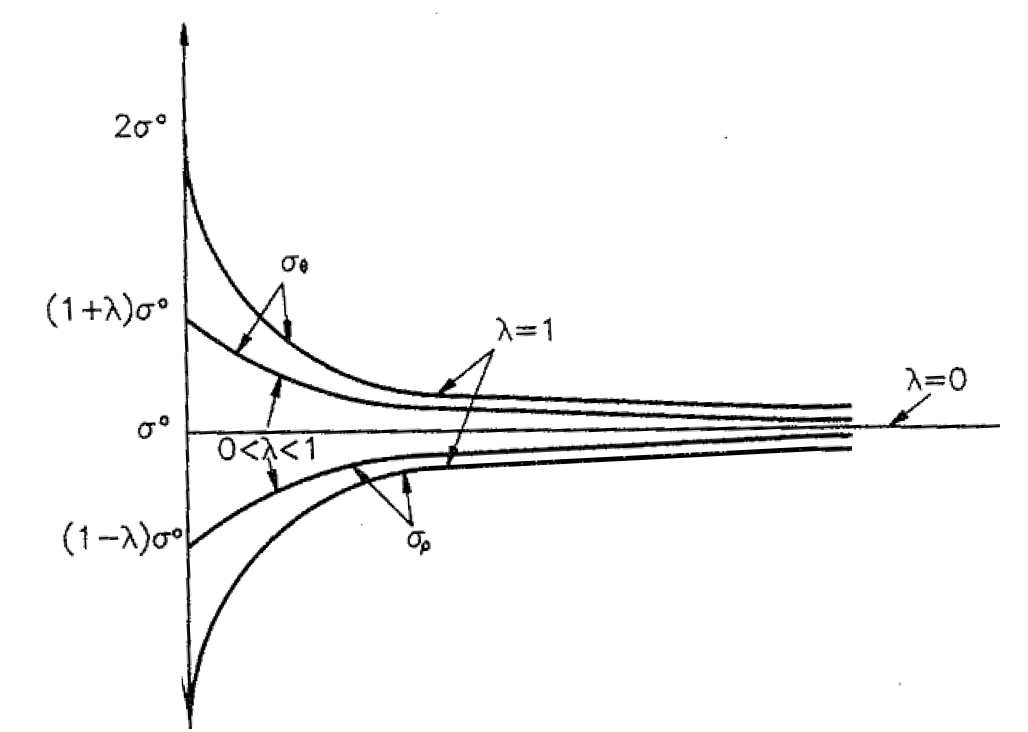
\includegraphics[height=3.5cm]{Results_sigmar.png}
    \caption{\scriptsize{Solution théorique des relations $\sigma_r(r)$ et $\sigma_{\theta}(r)$}}
    \label{Results_sigmar}
    \end{figure}
    
    Deuxième composante de la courbe caractéristique du massif : \[\sigma_r(r=R) = (1-\lambda)\sigma_0\]

\end{frame}




\begin{frame}{Distribution des contraintes}

\begin{figure}
\centering
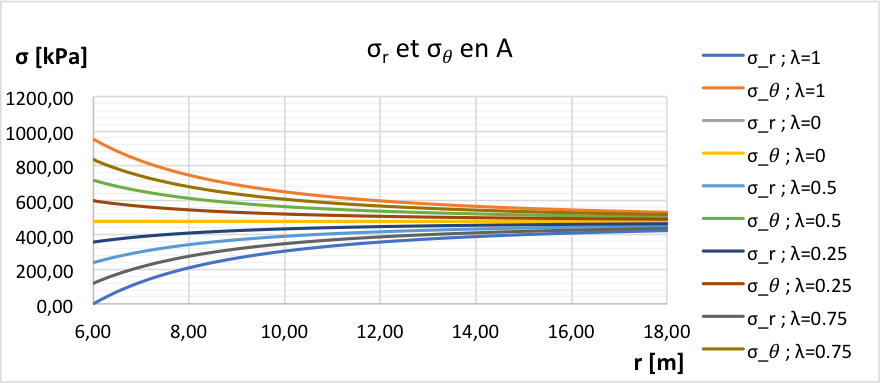
\includegraphics[width=8cm]{sig_A.png}
\end{figure}

\begin{figure}
\centering
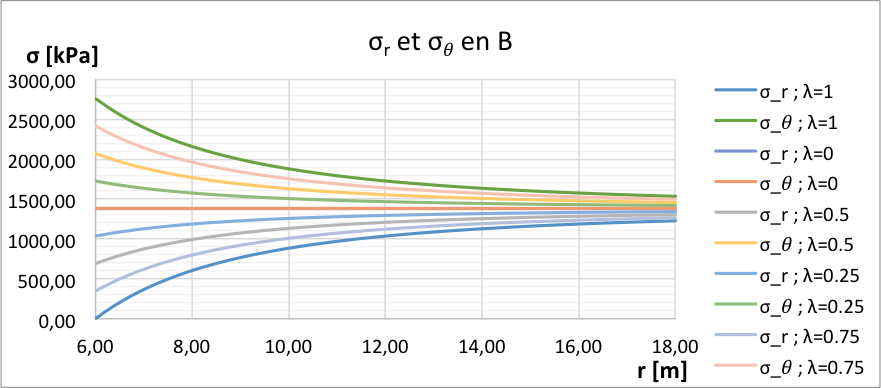
\includegraphics[width=8cm]{sig_B.png}
\end{figure}
    
\end{frame}
%on est à la périphérie du soutènement, on calcule sigma_r en fonction de lambda 
%alpha -> dépend de x / corrélation avec lambda : variation x de -2R à 4R est comme variation lambda 0 à 1

%loin dans confinement = soutènement mis trop tard ou pas nécessaire






\subsection{Chemins de contraintes p-q et $\sigma_r - \sigma_{\theta}$}



\begin{frame}{Chemins de contraintes}
  
\underline{Chemins de contraintes $p-q$}  

    \[\text{\textbf{Contraintes moyennes :}}\quad  p = \dfrac{\sigma_r + \sigma_{\theta}}{2}=\sigma_0\]
    \[\text{\textbf{Contraintes déviatoriques :}}\quad q=\sigma_{\theta} - \sigma_r=2\lambda\sigma_0\]

\vspace{0,5cm}
\underline{Chemins de contraintes $\sigma_r - \sigma_{\theta}$}      
   
    \[\sigma_r(r=R) = \left( 1 - \lambda \right) \sigma_0\quad \text{et}\quad \sigma_{\theta}(r=R) = \left( 1 + \lambda \right) \sigma_0\]
      
    $\rightarrow$ Contraintes radiales évoluent de manière \textbf{inversément proportionnelle} aux contraintes tangentielles\\
      
    \[\text{En}\;\lambda=0\;:\quad\sigma_r=\sigma_{\theta}=\sigma_0\]

\end{frame} 


\begin{frame}{Chemins de contraintes p-q}

\begin{figure}
\centering
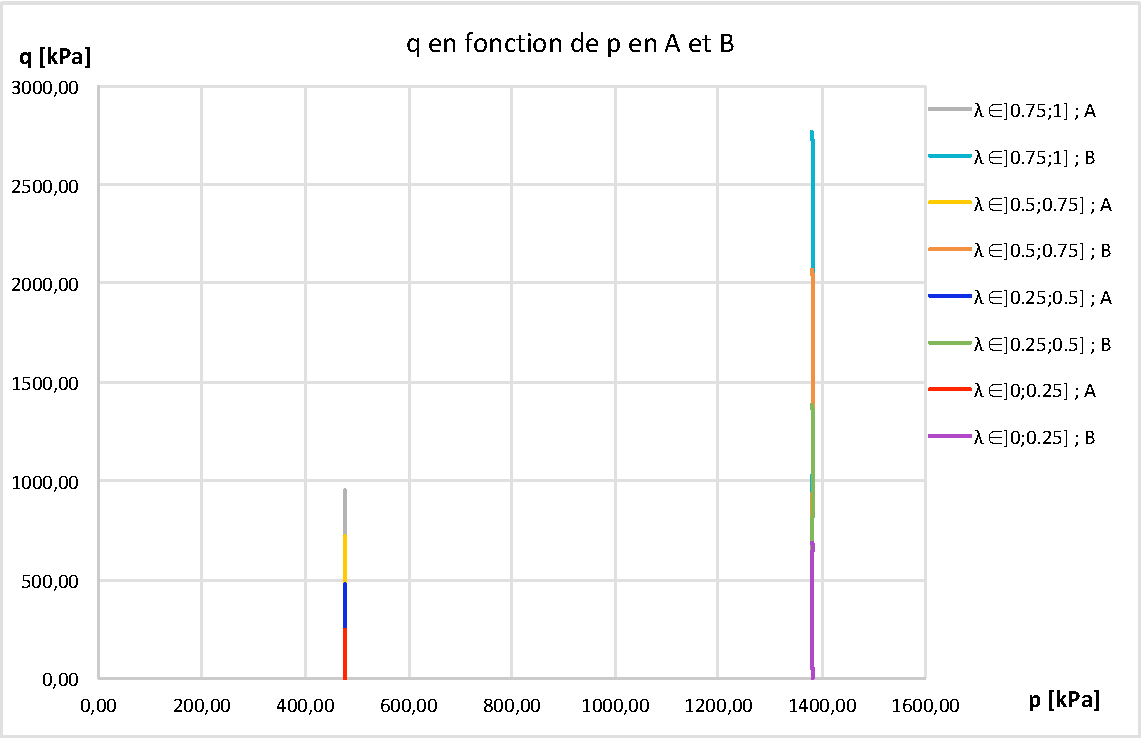
\includegraphics[width=10cm]{pq.pdf}
\end{figure}
    
\end{frame}

\begin{frame}{Chemins de contraintes $\sigma_r - \sigma_{\theta}$}
    
\begin{figure}
\centering
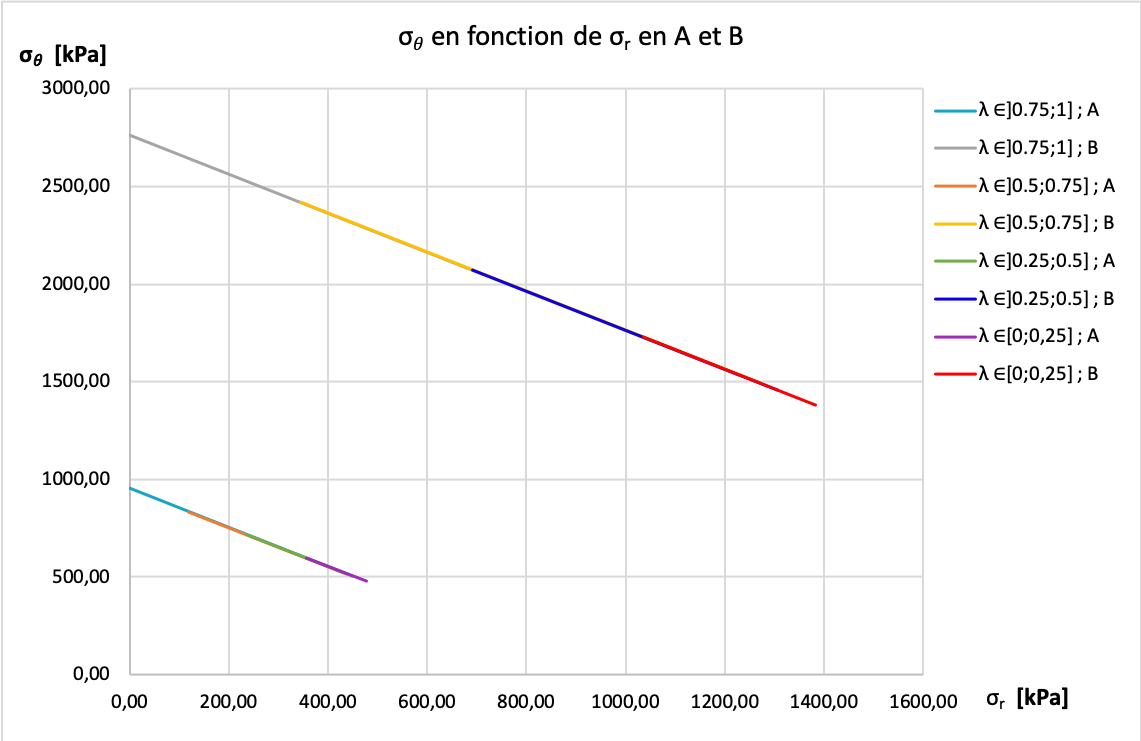
\includegraphics[width=10cm]{sig.png}
\end{figure}

\end{frame}




\subsection{Courbes caractéristiques}

\begin{frame}{Courbe caractéristique du soutènement}

\[\text{Si }\;x\in[-2R;4R]\;:\quad u_R(x)=\alpha(x)\dfrac{\sigma_0R}{2G}\]

\begin{figure}
\centering
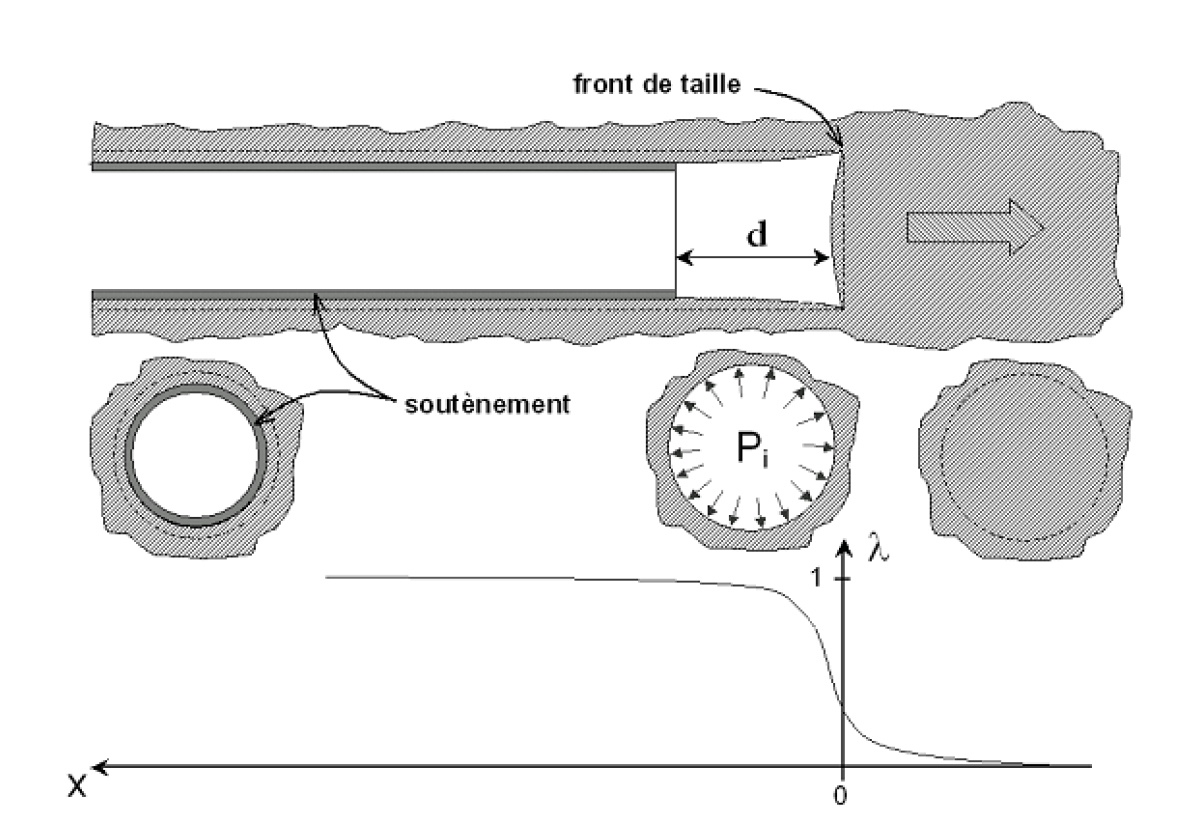
\includegraphics[height=4cm]{CourbeSout.png}
\caption{\scriptsize{Déplacements en paroi en fonction de la distance au front de taille}}
\label{CourbeSout}
\end{figure}
\vspace{-0.3cm}    
\[\alpha(x)=\alpha_0+(1-\alpha_0)\;a(x)\;\text{avec}\;\alpha_0=0,25\;\text{et}\;\forall x\geq0\]\[a(x)=1-\left[\dfrac{mR}{mR+x}\right]^2\;\text{avec}\;m=0,75\]
    
\end{frame}

\begin{frame}
\underline{Contraintes radiales :}\\
\[\text{Si}\;x<d\;:\quad \sigma_r(x)=0\]
\[\text{Si}\;x\in[d;4R]\;:\quad \sigma_r(x)=K_{sn}\dfrac{u_r(x)-u_r(d)}{R}\]
\[K_{sn}=\dfrac{E_b}{1-\nu_b^2}\dfrac{e_b}{R}\;\text{en paroi mince}\;\left(\dfrac{R}{e_b}>10\right)\]
    
    
\end{frame}

\begin{frame}{Courbes caractéristiques}
    
\begin{figure}
\centering
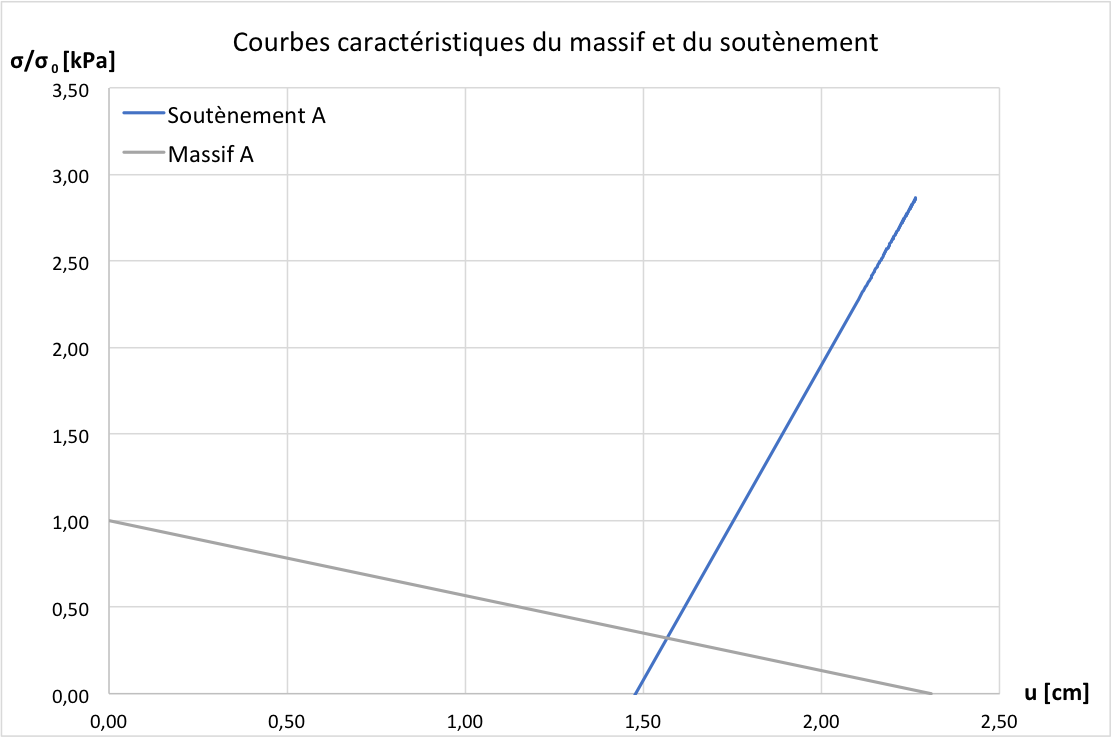
\includegraphics[width=9cm]{sig_u_A.png}
\end{figure}
\[\text{d=2m et e=20cm}\]
\end{frame}


\begin{frame}

\begin{figure}
\centering
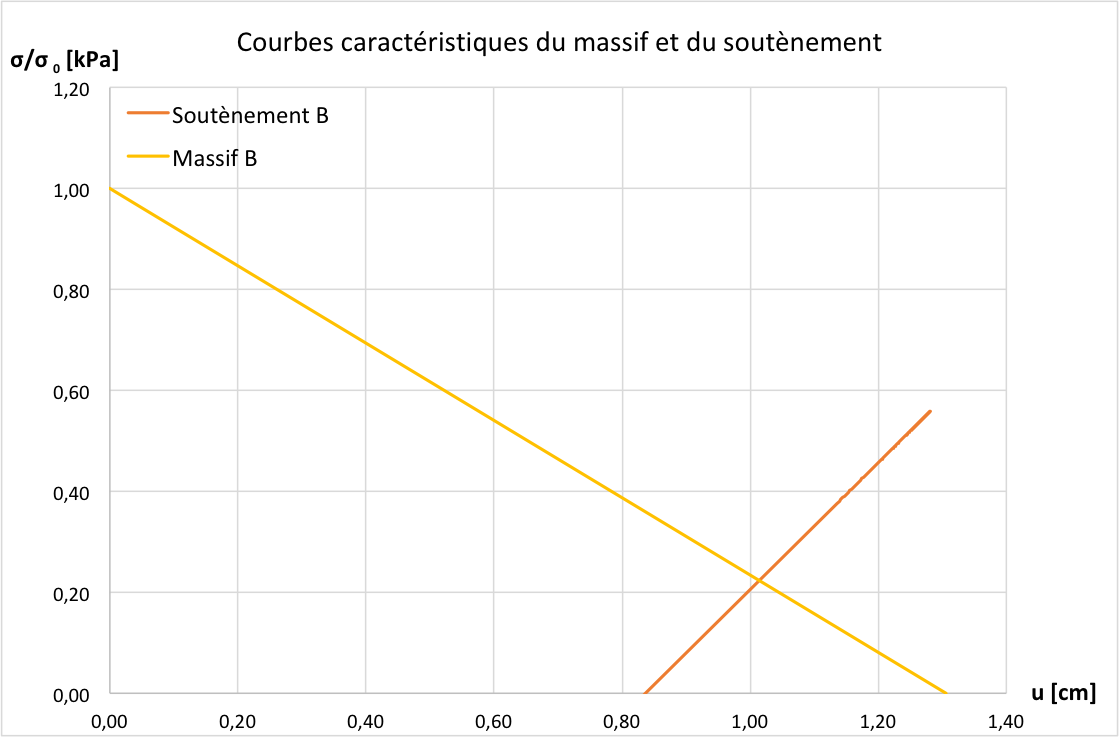
\includegraphics[width=9cm]{sig_u_B.png}
\end{figure}
\[\text{d=2m et e=20cm}\]

\end{frame}

\subsection{Variation des paramètres}

\begin{frame}{Variation de la distance du soutènement}

\begin{figure}
\centering
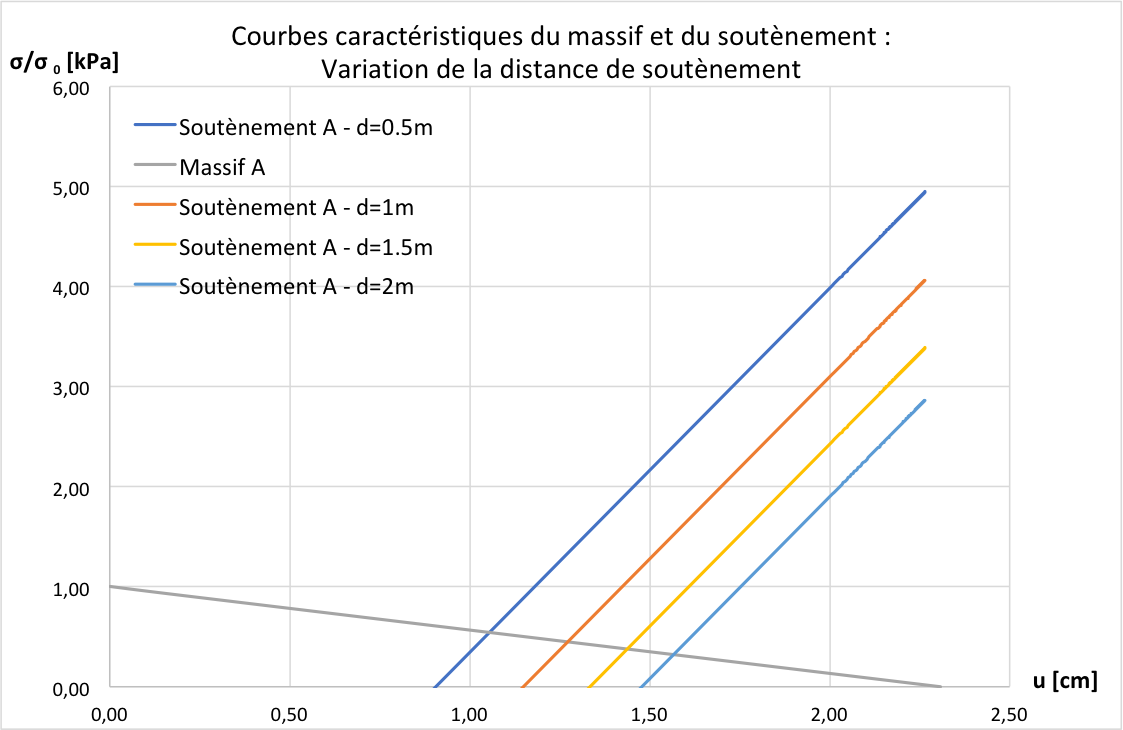
\includegraphics[width=10cm]{var_d.png}
\end{figure}

\end{frame}


\begin{frame}{Variation de l'épaisseur du soutènement}

\begin{figure}
\centering
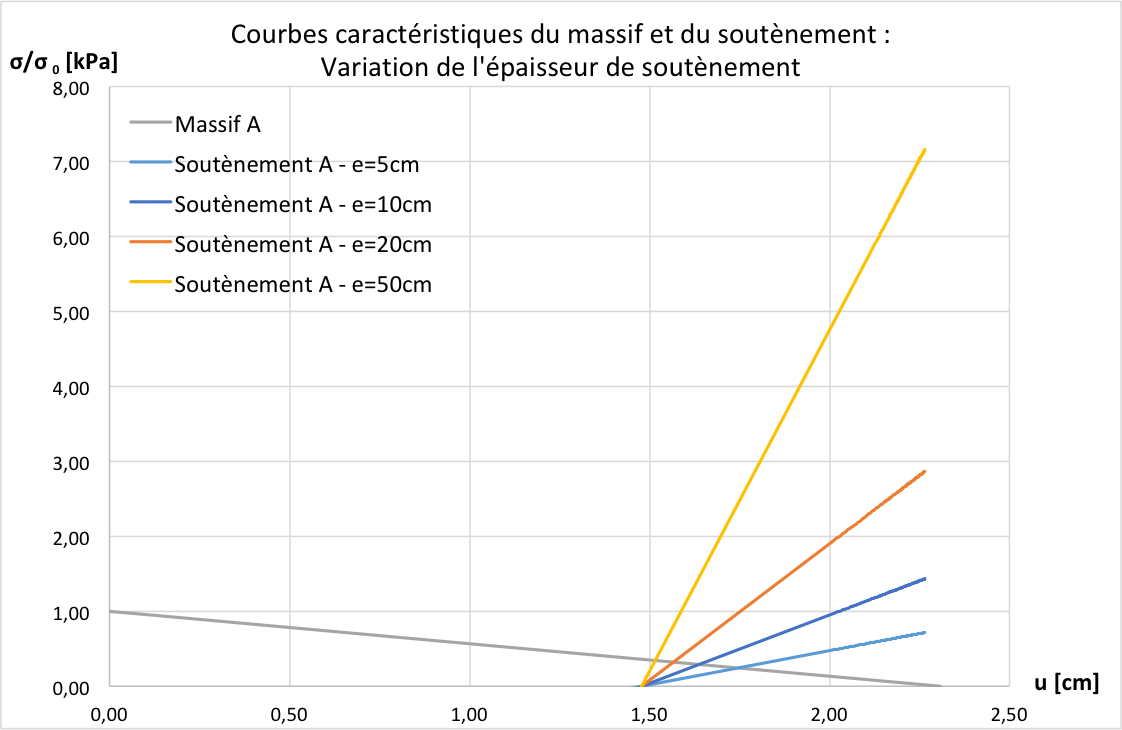
\includegraphics[width=10cm]{var_e.png}
\end{figure}

\end{frame}




\section{Étude élastoplastique}

\subsection{Critère de Mohr-Coulomb et comportement élastoplastique}

\begin{frame}{Critère de Mohr-Coulomb}

\[\tau=\sigma_n\;\tan\phi+c\]
\[\longrightarrow \sigma_c=\sigma_{\theta}-K_p\sigma_r\]

\begin{figure}
    \centering
    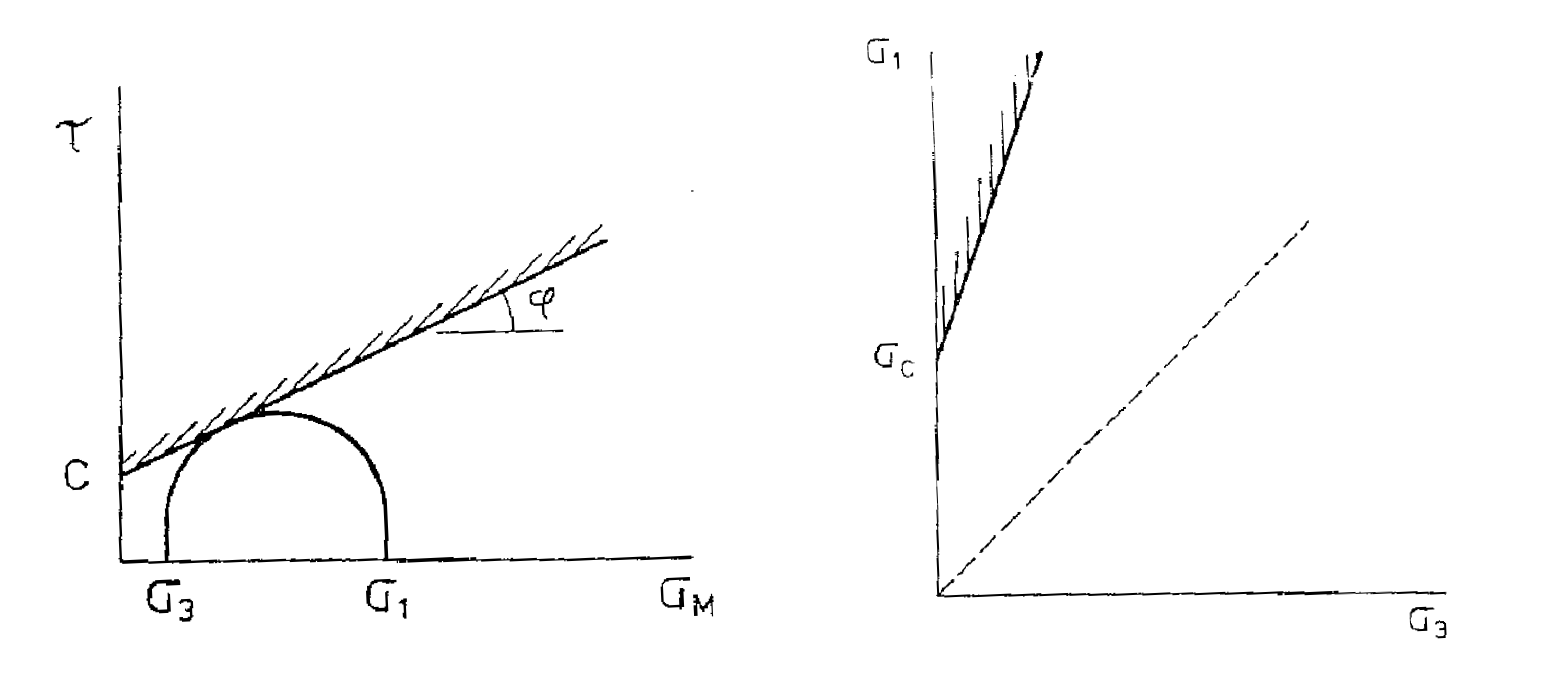
\includegraphics[height=4cm]{MohrCoulomb.png}
    \caption{\scriptsize{Modèle de Mohr-Coulomb}}
    \label{MohrCoulomb}
\end{figure}
\vspace{-0.3cm}
\[K_p=\dfrac{1+\sin\phi}{1-\sin\phi}\;\text{et}\;\sigma_c=\dfrac{2c\;\cos\phi}{1-\sin\phi}\]
    
\end{frame}



\begin{frame}{Comportement élastoplastique}

Comportement \textbf{plastique parfait} (sans écrouissage ni adoucissement) :\[\lambda_e=\dfrac{1}{K_p+1}\left[K_p-1+\dfrac{\sigma_c}{\sigma_0}\right]\]

\[\text{Rayon plastique :}\quad R_p=\left\{\begin{array}{l}R\;\text{si}\;\lambda\leq\lambda_e\\ \\
R\left[\dfrac{2\lambda_e}{(K_p+1)\lambda_e-(K_p-1)\lambda}\right]^{1/(K_p-1)} \;\text{si}\;\lambda>\lambda_e\end{array}\right.\]

\begin{figure}
    \centering
    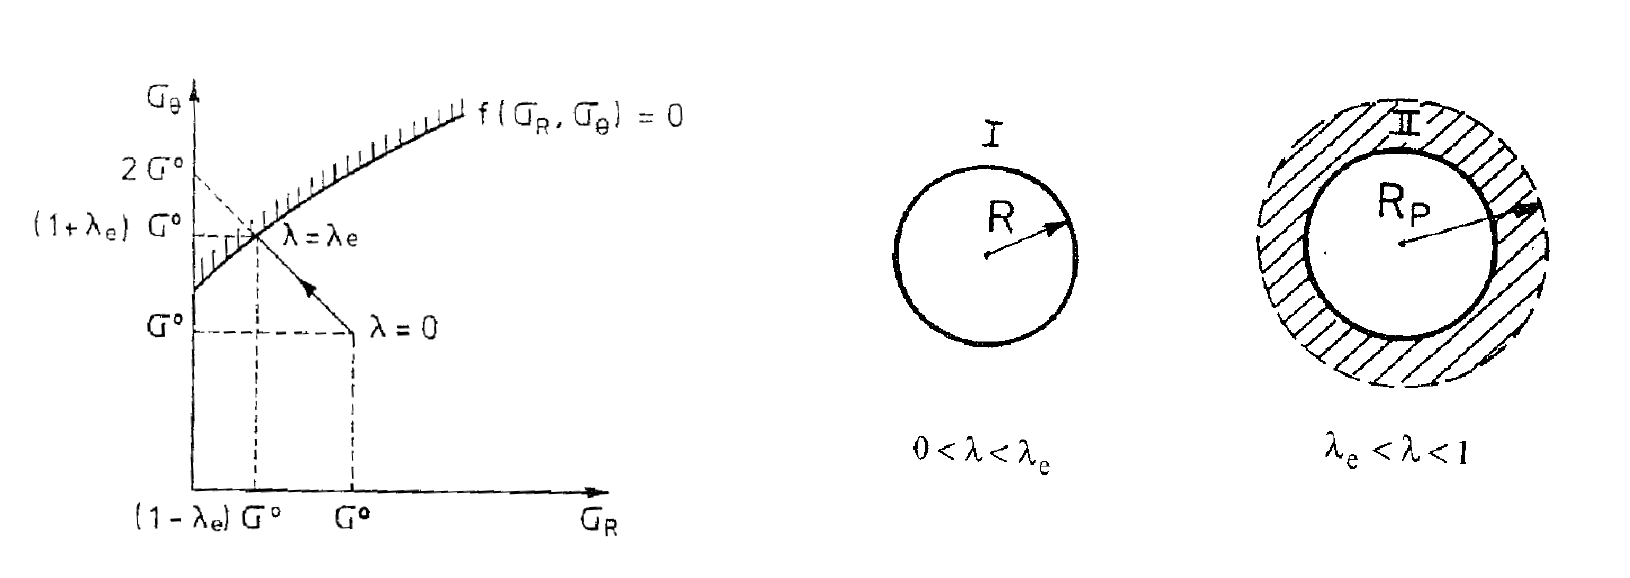
\includegraphics[height=3cm]{RpTh.png}
    \caption{\scriptsize{Évolution du rayon plastique}}
    \label{RpTh}
\end{figure}
    
\end{frame}

\subsection{Déplacement du massif}

\begin{frame}{Déplacement du massif}

\[u_r(r)=\left\{\begin{array}{l}
\lambda\dfrac{R^2}{r}\dfrac{\sigma_0}{2G}\;\text{si}\;\lambda\leq\lambda_e\\\\
\dfrac{\lambda_e\sigma_0r}{2G}\left(F_1+F_2\left(\dfrac{r}{R_p}\right)^{K_p-1}+F_3\left(\dfrac{R_p}{r}\right)^{K+1}\right)\;\text{si}\;\lambda>\lambda_e\;\text{et}\;r\leq R_p\\\\
\lambda_e\dfrac{R_p^2}{r}\dfrac{\sigma_0}{2G}\;\text{si}\;\lambda>\lambda_e\;\text{et}\;r> R_p\end{array}\right.\]

où $F_1$, $F_2$, $F_3$ et $K$ sont des paramètres dépendant de $\nu$, $K_p$ et $\psi$.\\

On a par ailleurs calculé : \[\lambda_{e,\text{couche A}} = 0,39\]
\[\lambda_{e,\text{couche B}} = 0,52\]


    
\end{frame}


\begin{frame}{Déplacement du massif}
    
    \begin{columns}
    \begin{column}{0.5\textwidth}
\begin{figure}
\centering
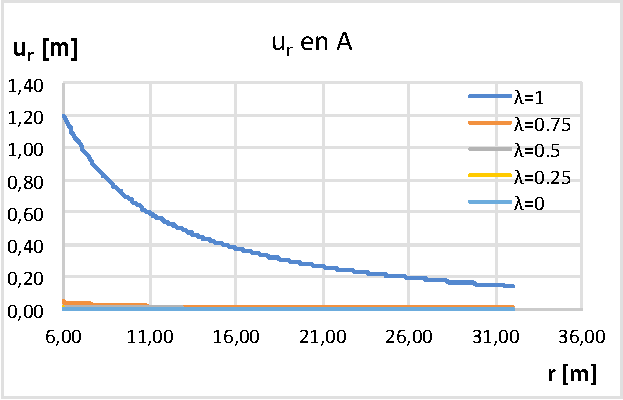
\includegraphics[width=5.5cm]{ur_A2.pdf}
%\caption{Déplacement du massif en A}
\end{figure}
    \end{column}
    
    \begin{column}{0.5\textwidth}
\begin{figure}
\centering
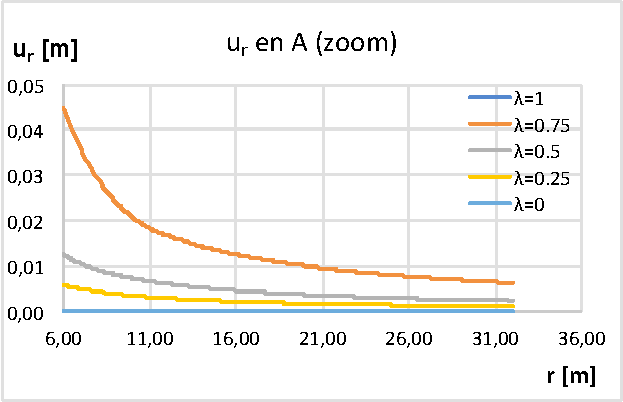
\includegraphics[width=5.5cm]{ur_A_zoom.pdf}
%\caption{Déplacement du massif en B}
\end{figure}
    \end{column}
    \end{columns}
    
    \begin{figure}
\centering
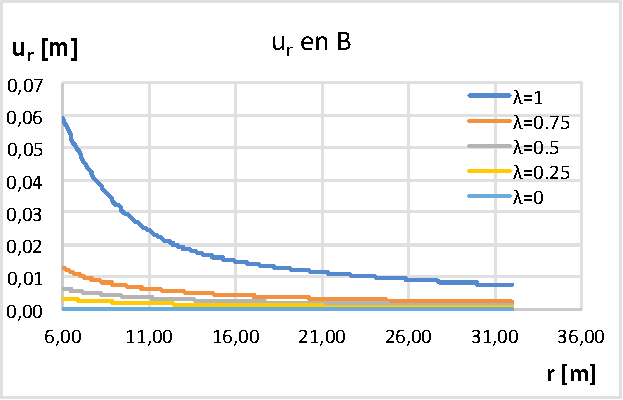
\includegraphics[width=5.5cm]{ur_B2.pdf}
%\caption{Déplacement du massif en B}
\end{figure}

\end{frame}

\begin{frame}{Rayon plastique}

\[\text{Plus $\lambda$ est grand, et plus $R_p$ est grand $\longrightarrow$ Grands déplacements}\]

\begin{figure}
\centering
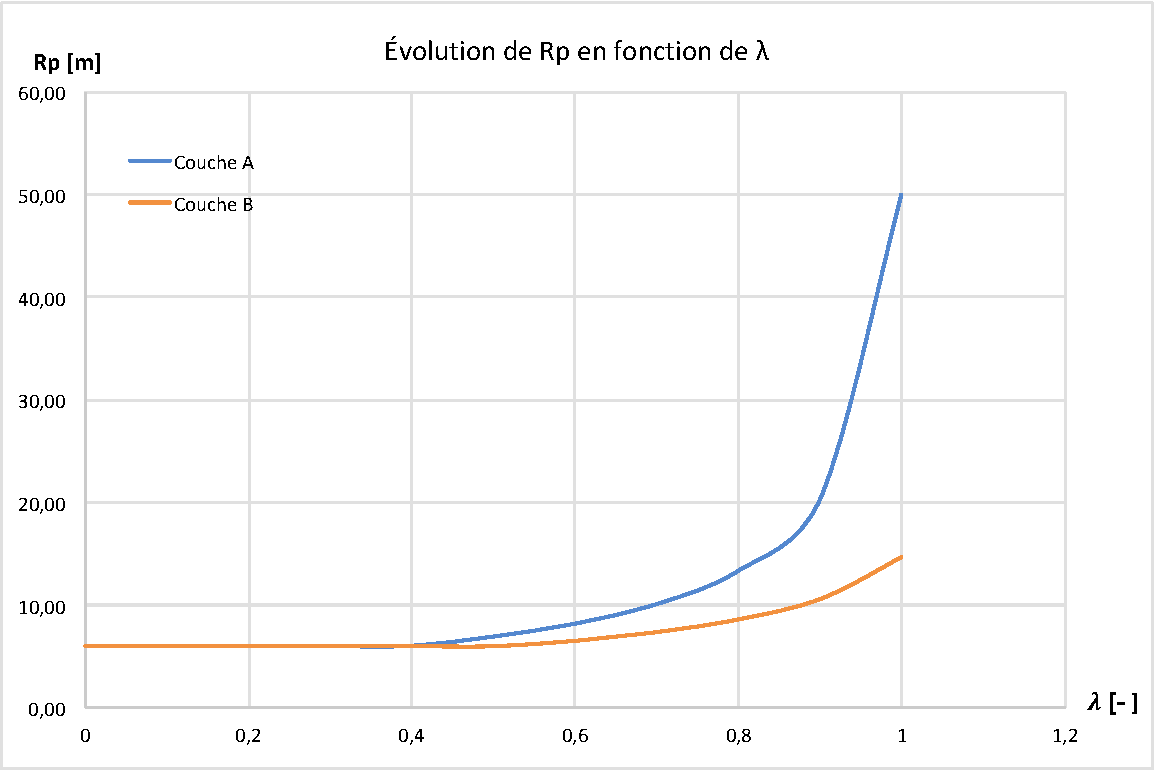
\includegraphics[width=10cm]{RPlambda.pdf}
\end{figure}
    
\end{frame}

\subsection{Distribution des contraintes}

\begin{frame}{Distribution des contraintes}

\begin{align*}
\sigma_r(r)&=\left\{\begin{array}{l}
\left(1-\lambda\dfrac{R^2}{r^2}\right)\sigma_0\;\text{si}\;\lambda\leq\lambda_e\\\\
\left(\dfrac{\sigma_0}{K_p-1}\right)\left(2\lambda_e\left(\dfrac{r}{R_p}\right)^{K_p-1}-\dfrac{\sigma_c}{\sigma_0}\right)\;\text{si}\;\lambda>\lambda_e\;\text{et}\;r\leq R_p\\\\
\left(1-\lambda_e\dfrac{R_p^2}{r^2}\right)\sigma_0\;\text{si}\;\lambda>\lambda_e\;\text{et}\;r> R_p\end{array}\right.\\\\
\sigma_{\theta}(r)&=\left\{\begin{array}{l}
\left(1+\lambda\dfrac{R^2}{r^2}\right)\sigma_0\;\text{si}\;\lambda\leq\lambda_e\\\\
\sigma_c+K_p\;\sigma_{r,plast}\;\text{si}\;\lambda>\lambda_e\;\text{et}\;r\leq R_p\\\\
\left(1+\lambda_e\dfrac{R_p^2}{r^2}\right)\sigma_0\;\text{si}\;\lambda>\lambda_e\;\text{et}\;r> R_p\end{array}\right.
\end{align*}
\end{frame}

\begin{frame}{Distribution des contraintes}

\begin{figure}
    \centering
    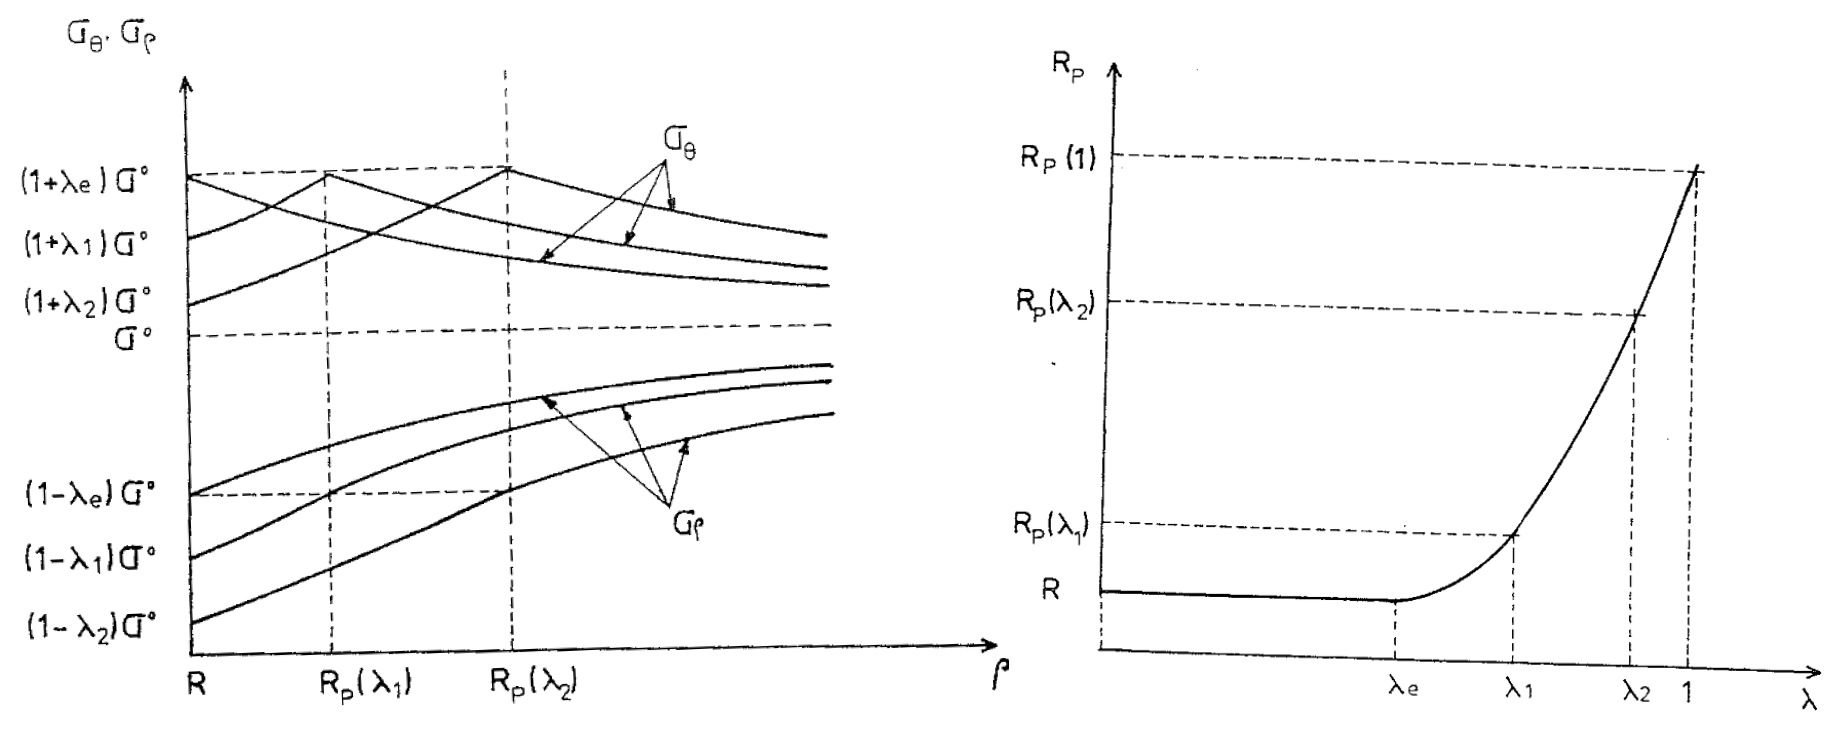
\includegraphics[height=4cm]{SigTresca.png}
    \caption{\scriptsize{Distribution des contraintes pour le modèle de Tresca}}
    \label{SigTresca}
\end{figure}
\vspace{-0.2cm}
Dans notre cas (Mohr-Coulomb) : \[\sigma_{\theta}-\sigma_r=2c\longrightarrow \sigma_{\theta}-K_p\sigma_r=\sigma_c\]


\end{frame}



\begin{frame}{Distribution des contraintes}

\begin{figure}
\centering
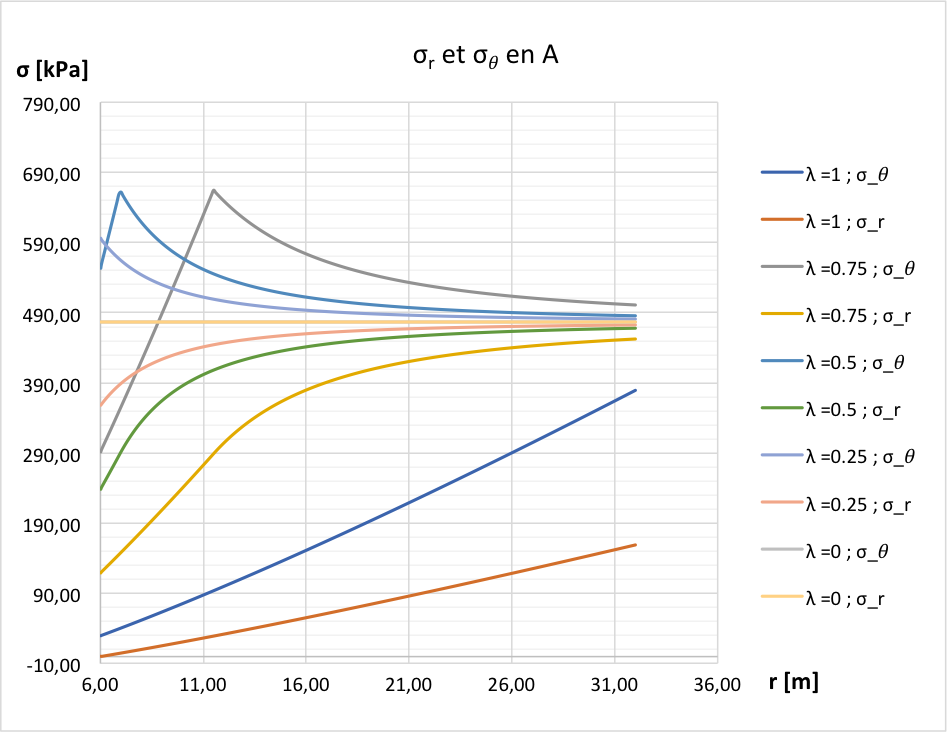
\includegraphics[width=9cm]{sig_A2.png}
\end{figure}
\[\text{Pic en }r=R_p\]
\end{frame}


\begin{frame}{Distribution des contraintes}

\begin{figure}
\centering
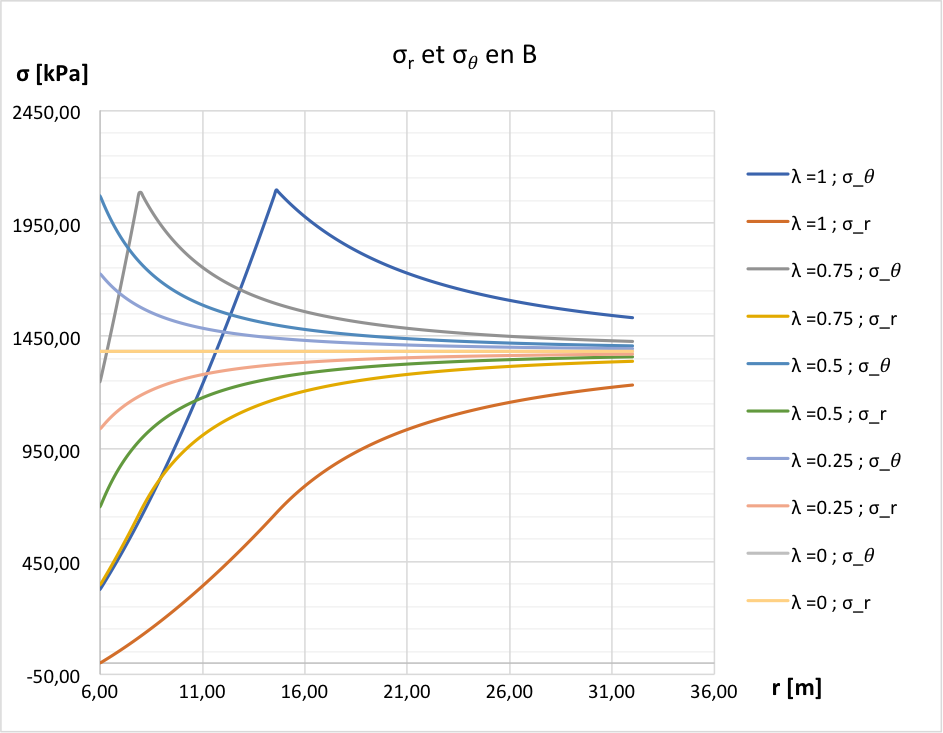
\includegraphics[width=9cm]{sig_B2.png}
\end{figure}
    
\end{frame}











\subsection{Chemins de contraintes p-q et $\sigma_r - \sigma_{\theta}$}


\begin{frame}{Chemins de contraintes p-q}

\begin{figure}
\centering
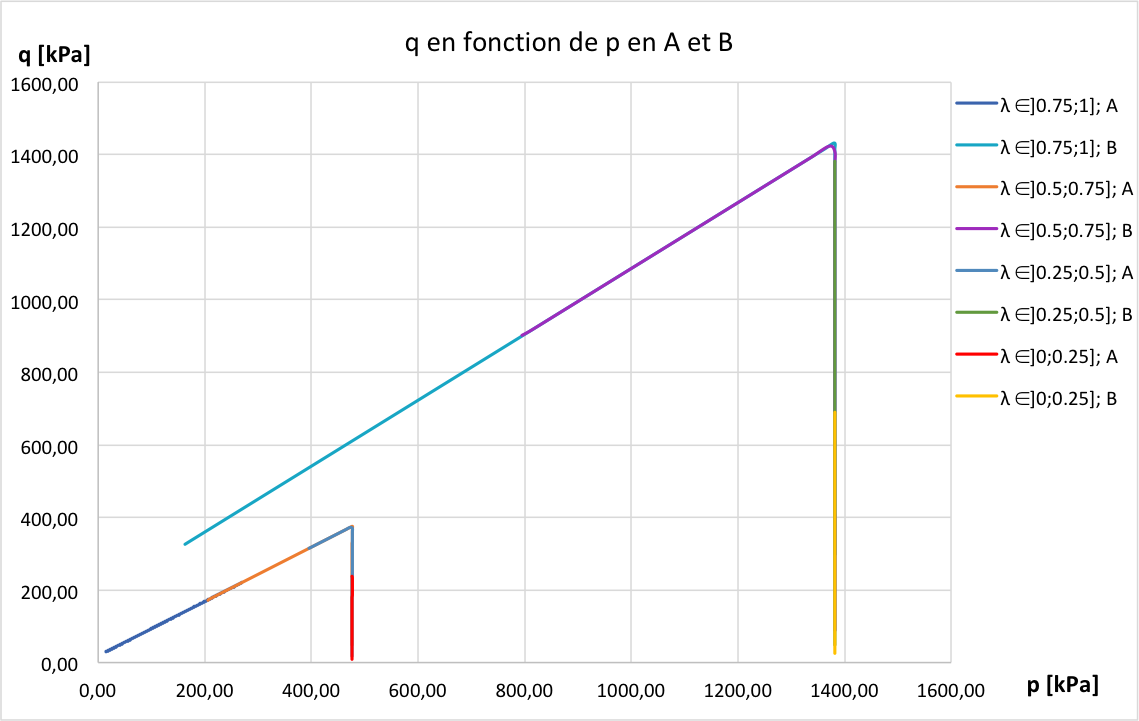
\includegraphics[width=10cm]{pq2.png}
\end{figure}
    
\end{frame}





\begin{frame}{Chemins de contraintes $\sigma_r - \sigma_{\theta}$}
    
\begin{figure}
\centering
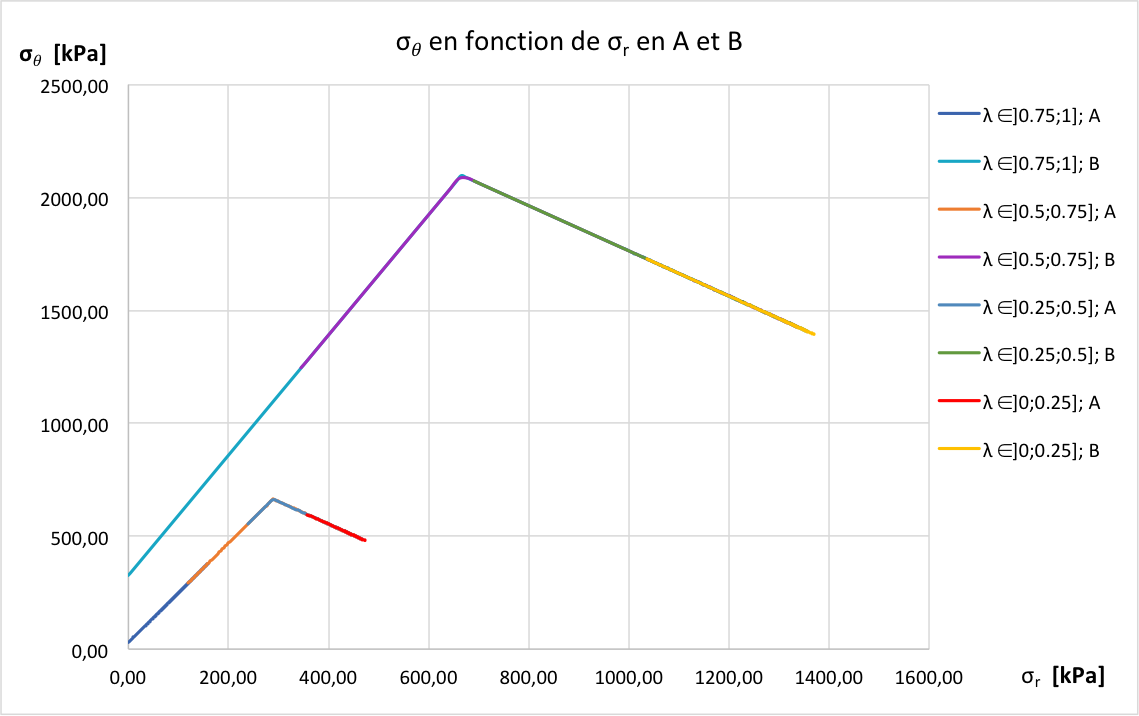
\includegraphics[width=10cm]{sig2.png}
\end{figure}

\end{frame}



\subsection{Courbes caractéristiques}

\begin{frame}{Courbe caractéristique du massif}
    
    \begin{align*}
    u_r(r=R)&=\left\{\begin{array}{l}
    \dfrac{\lambda\sigma_0R}{2G}\;\text{si}\;\lambda\leq\lambda_e\\\\
    \dfrac{\lambda_e\sigma_0R}{2G}\left(F_1+F_2\left(\dfrac{R}{R_p}\right)^{K_p-1}+F_3\left(\dfrac{R_p}{R}\right)^{K+1}\right)\;\text{si}\;\lambda>\lambda_e\end{array}\right.\\\\
    \sigma_r(r=R)&=\left\{\begin{array}{l}
    (1-\lambda)\sigma_0\;\text{si}\;\lambda\leq\lambda_e\\\\
    \left(\dfrac{\sigma_0}{K_p-1}\right)\left(2\lambda_e\left(\dfrac{R}{R_p}\right)^{K_p-1}-\dfrac{\sigma_c}{\sigma_0}\right)\;\text{si}\;\lambda>\lambda_e\end{array}\right.\\\\
    \sigma_{\theta}(r=R)&=\left\{\begin{array}{l}
    (1+\lambda)\sigma_0\;\text{si}\;\lambda\leq\lambda_e\\\\
    \sigma_c+K_p\;\sigma_{r,plast}\;\text{si}\;\lambda>\lambda_e\end{array}\right.
    \end{align*}
    
\end{frame}

\begin{frame}{Courbe caractéristique du soutènement}

\underline{Déplacement radial :}\\
\[\text{Si }\;x\in[-2R;4R]\;:\quad u_R(x)=\dfrac{1}{\xi}\alpha(x)\dfrac{\sigma_0R}{2G}\]\vspace{0.7cm}


\[\dfrac{1}{\xi} = \lambda_e\left(\dfrac{R_{p,max}}{R}\right)^{K+1}\;\text{avec}\;R_{p,max}=R_p(\lambda=1)\]
\[\alpha(x)=\alpha_0+(1-\alpha_0)\;a(x)\;\text{avec}\;\alpha_0=0,25\;\text{et}\;\forall x\geq0\]\[a(x)=1-\left[\dfrac{mR}{mR+x\xi}\right]^2\;\text{avec}\;m=0,75\]
    
\end{frame}


\begin{frame}
\underline{Contraintes radiales :}\\

\[\text{Si}\;x<d\;:\quad \sigma_r(x)=0\]
\[\text{Si}\;x\in[d;4R]\;:\quad \sigma_r(x)=K_{sn}\dfrac{u_r(x)-u_r(d)}{R}\]
\[K_{sn}=\dfrac{E_b}{1-\nu_b^2}\dfrac{e_b}{R}\;\text{en paroi mince}\;\left(\dfrac{R}{e_b}>10\right)\]
    
\end{frame}

\begin{frame}{Courbes caractéristiques}
    
\begin{figure}
\centering
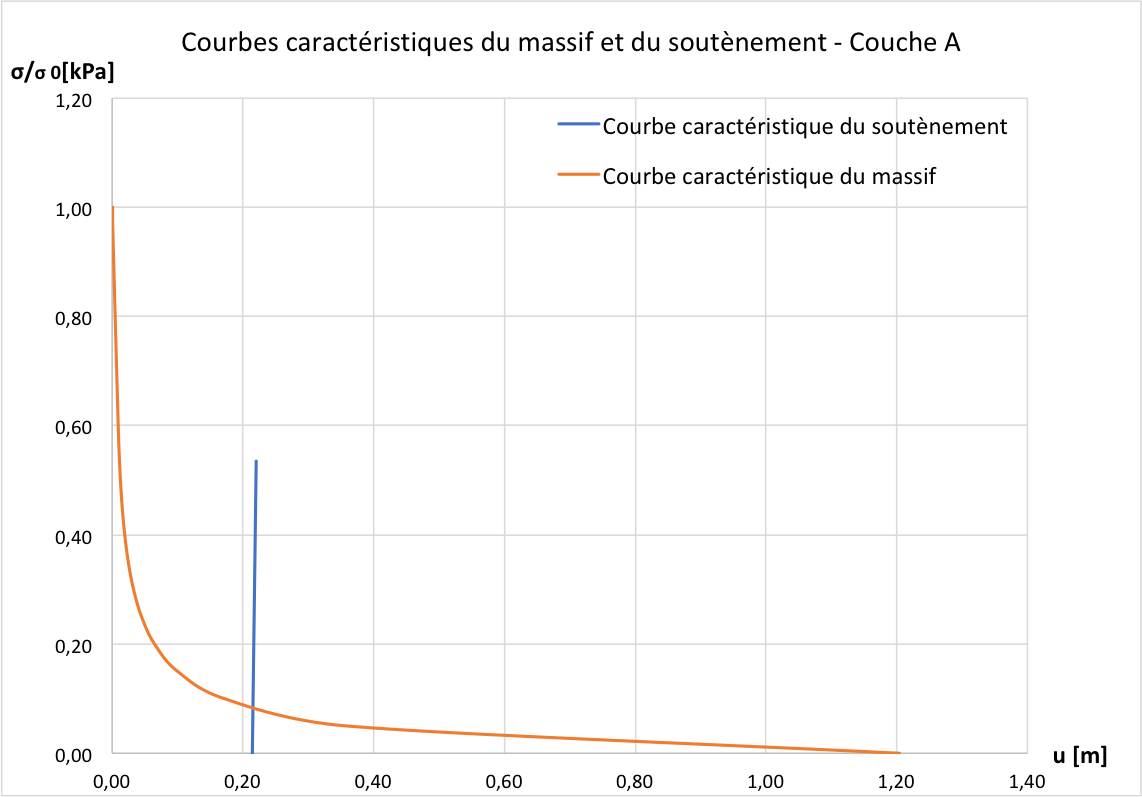
\includegraphics[width=10cm]{sig_u_A2.png}
\end{figure}
\[d=2\text{m et }e=5\text{cm}\]
\end{frame}


\begin{frame}{Courbes caractéristiques}

\begin{figure}
\centering
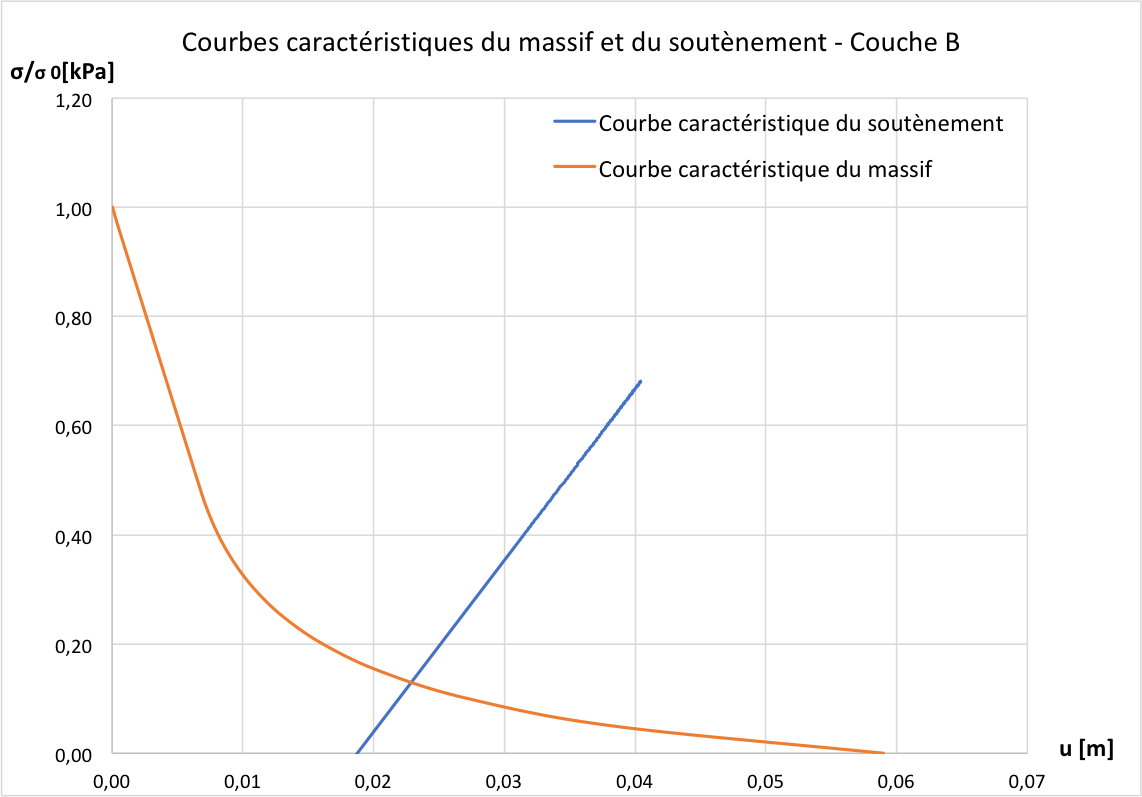
\includegraphics[width=10cm]{sig_u_B2.png}
\end{figure}
\[d=2\text{m et }e=5\text{cm}\]
\end{frame}





\subsection{Variation des paramètres}

\begin{frame}{Variation de l'épaisseur du soutènement}

\begin{figure}
\centering
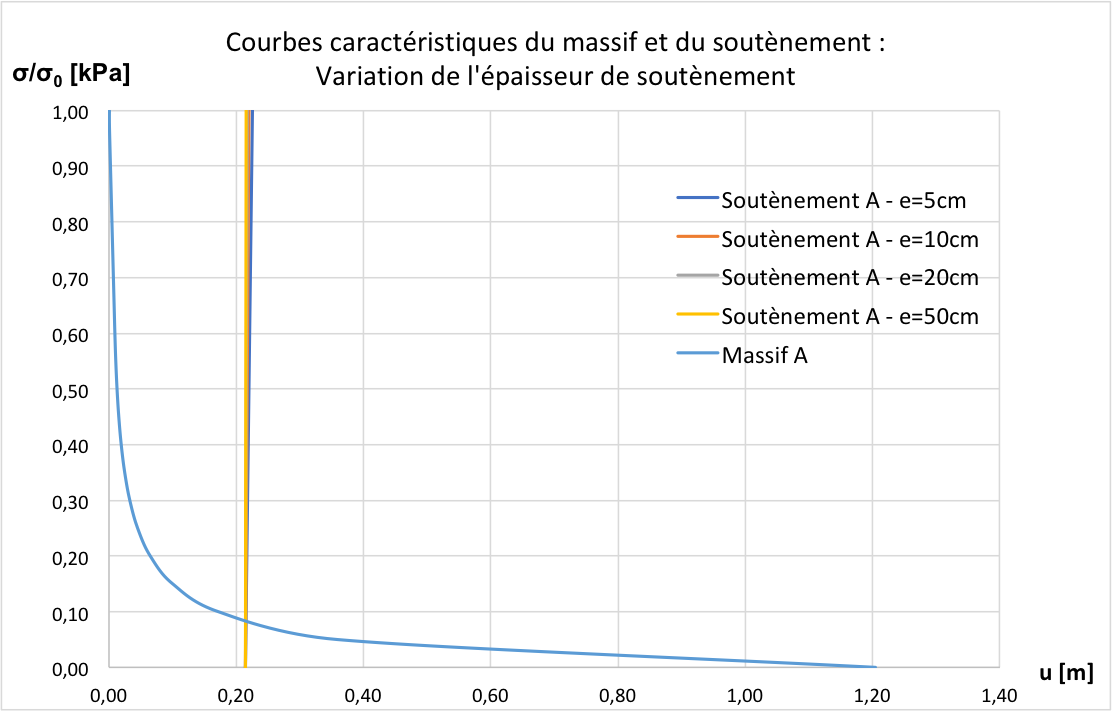
\includegraphics[width=10cm]{var_eA.png}
\end{figure}
\[d=2\text{m}\]    
\end{frame}

\begin{frame}{Variation de l'épaisseur du soutènement}

\begin{figure}
\centering
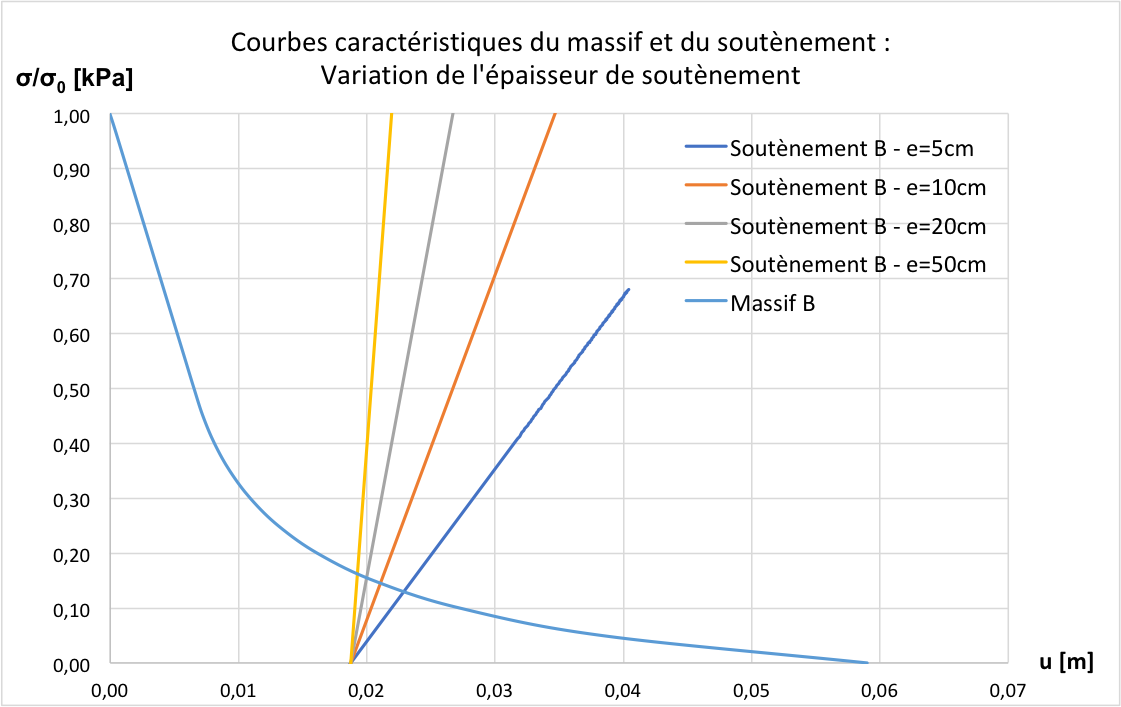
\includegraphics[width=10cm]{var_eB.png}
\end{figure}
\[d=2\text{m}\]
\end{frame}


\begin{frame}{Variation de la distance du soutènement}
    
\begin{figure}
\centering
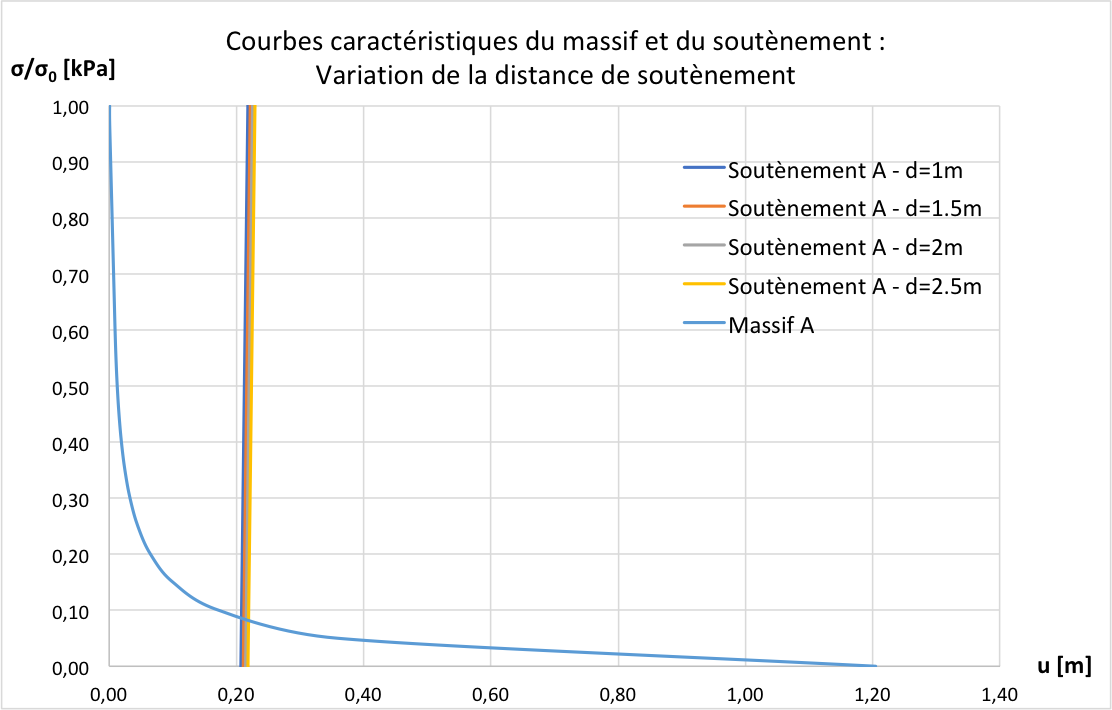
\includegraphics[width=10cm]{var_dA.png}
\end{figure}
\[e=5\text{cm}\]
\end{frame}



\begin{frame}{Variation de la distance du soutènement}
    
\begin{figure}
\centering
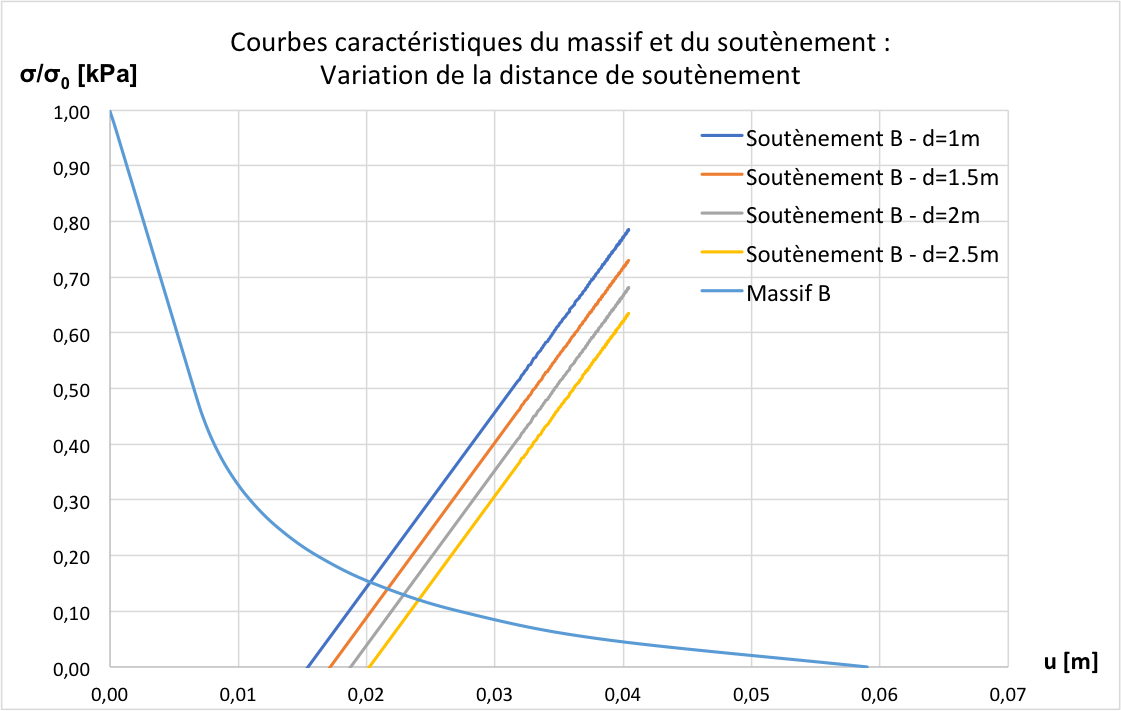
\includegraphics[width=10cm]{var_dB.png}
\end{figure}
\[e=5\text{cm}\]
\end{frame}



\begin{frame}{Variation du module de rigidité}

\begin{figure}
\centering
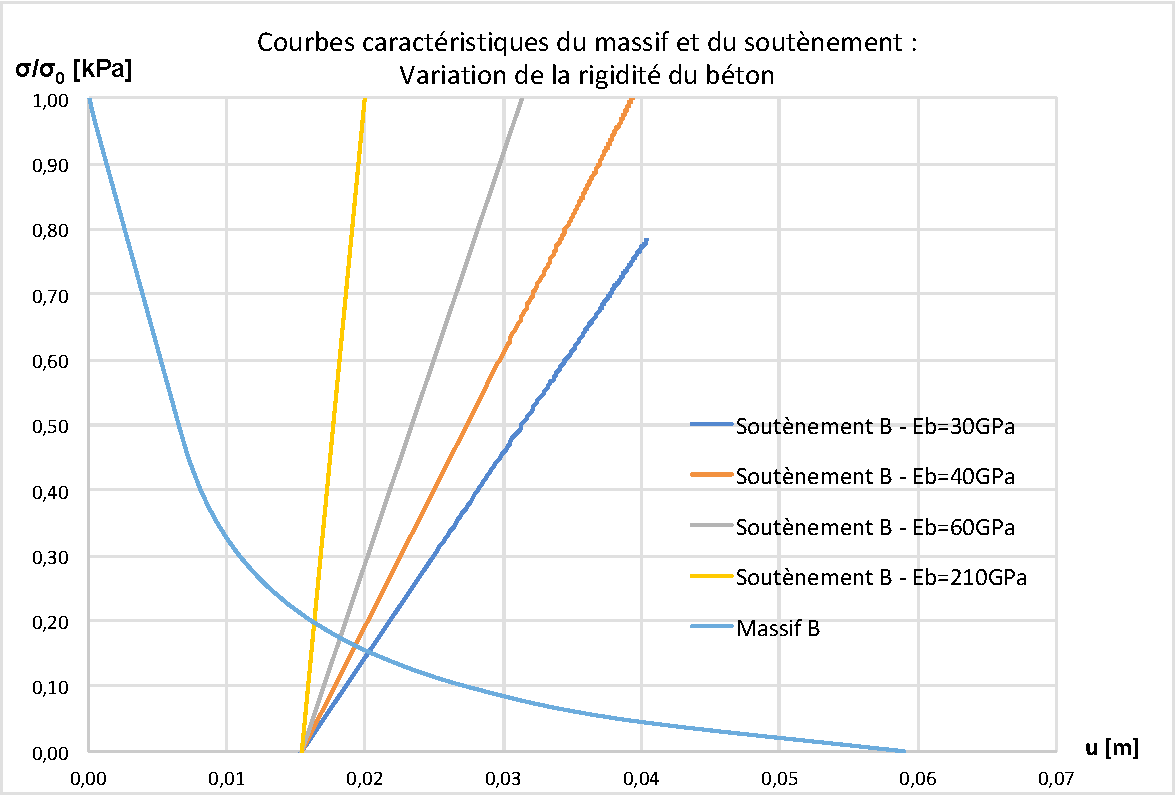
\includegraphics[width=10cm]{var_EbB.pdf}
\end{figure}
\[d=1\text{m et }e=5\text{cm}\]
\end{frame}

\begin{frame}{Variation de la cohésion dans le massif}
\begin{figure}
\centering
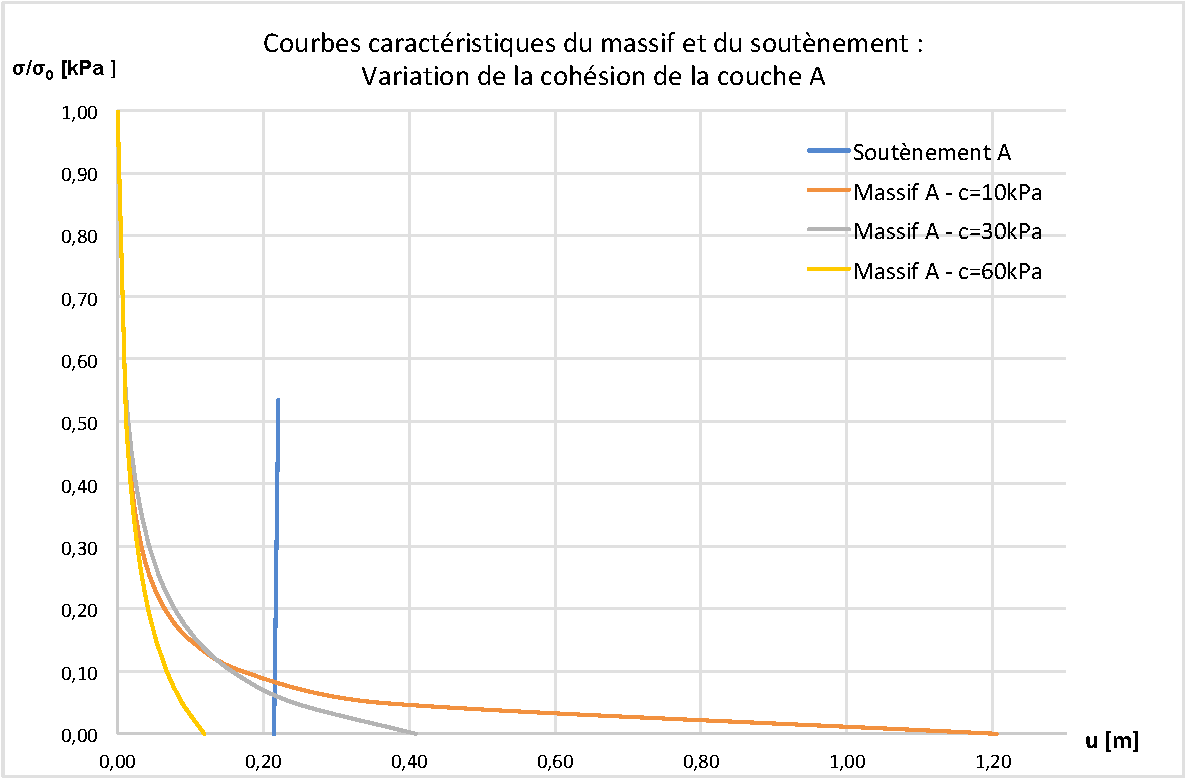
\includegraphics[width=10cm]{var_cA.pdf}
\end{figure}
\[d=2\text{m et }e=5\text{cm}\]
\end{frame}

\begin{frame}{Variation de l'angle de frottement dans le massif}
\begin{figure}
\centering
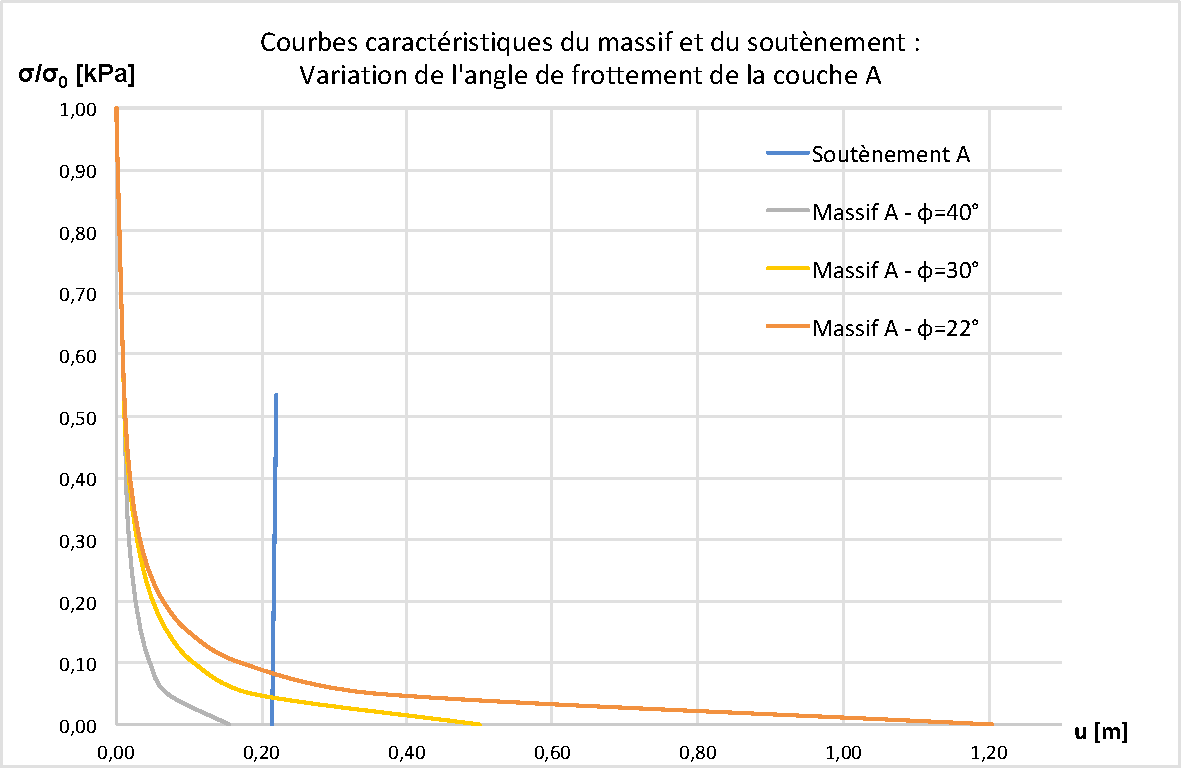
\includegraphics[width=10cm]{phi_A.pdf}
\end{figure}
\[d=2\text{m et }e=5\text{cm}\]    
\end{frame}

\begin{frame}{Variation du rayon de plasticité $R_p$}

\begin{figure}
\centering
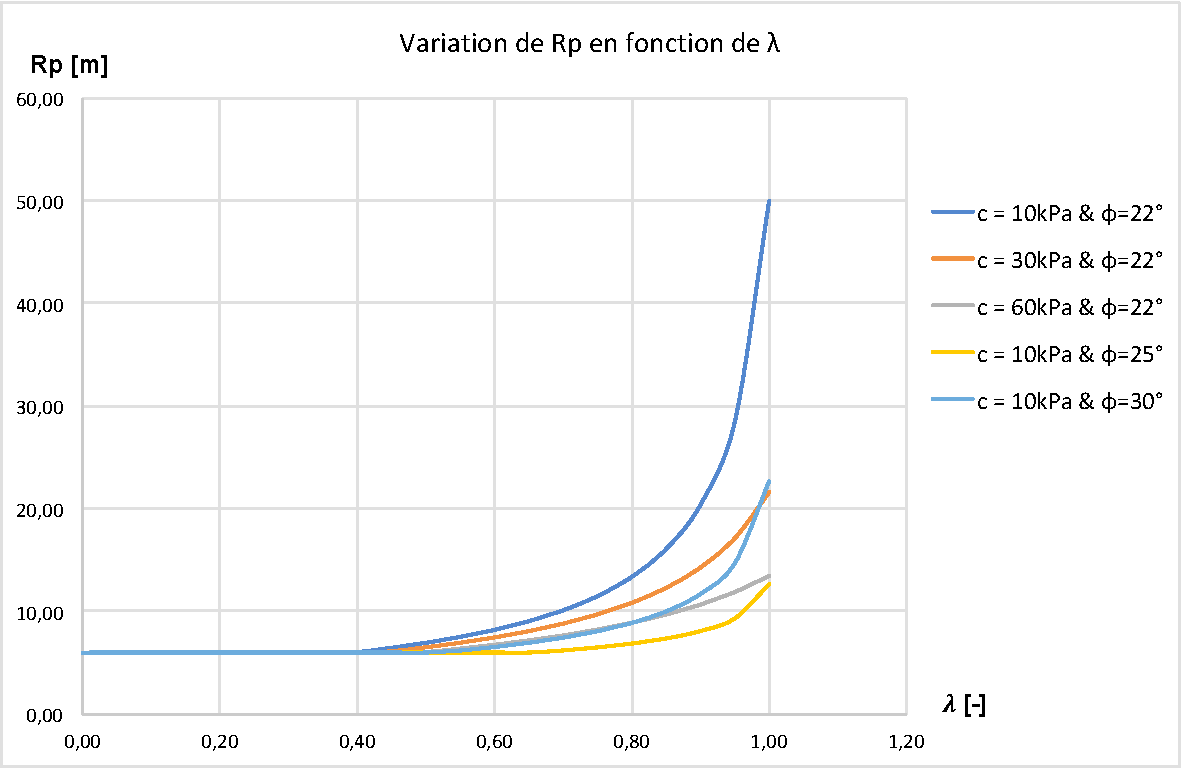
\includegraphics[width=10cm]{Rp.pdf}
\end{figure}
\[d=2\text{m et }e=5\text{cm}\]    
\end{frame}


\section{Dimensionnement}

\begin{frame}{Dimensionnement}
\begin{center}
Dimensionnement pour limiter $u_r(x)$ à 5 cm : \textbf{impossible} en A\\\vspace{0.5cm}
$\longrightarrow$ Accepter 20cm de déplacement OU Soutènement en voûtes parapluies
\end{center}
\end{frame}

\begin{frame}{Dimensionnement}

\begin{figure}
\centering
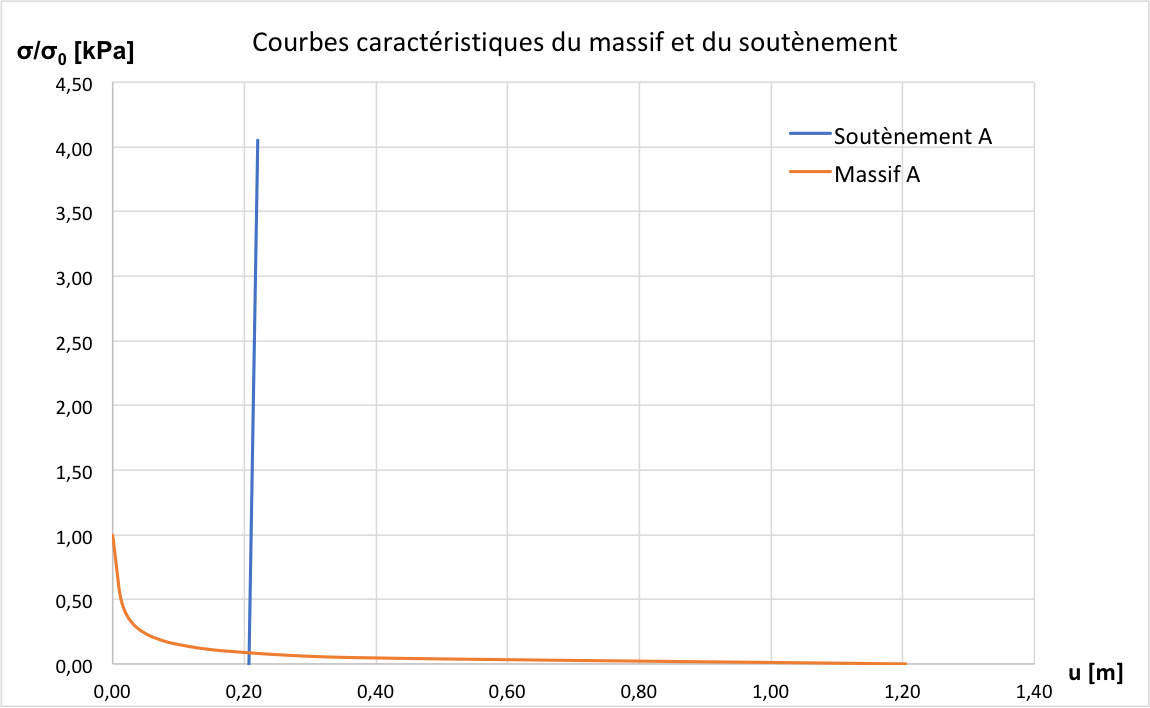
\includegraphics[width=10cm]{dimA.png}
\end{figure}
    \[d=1\text{m et }e=5\text{cm}\] 
\end{frame}



\begin{frame}{Dimensionnement}

\begin{figure}
\centering
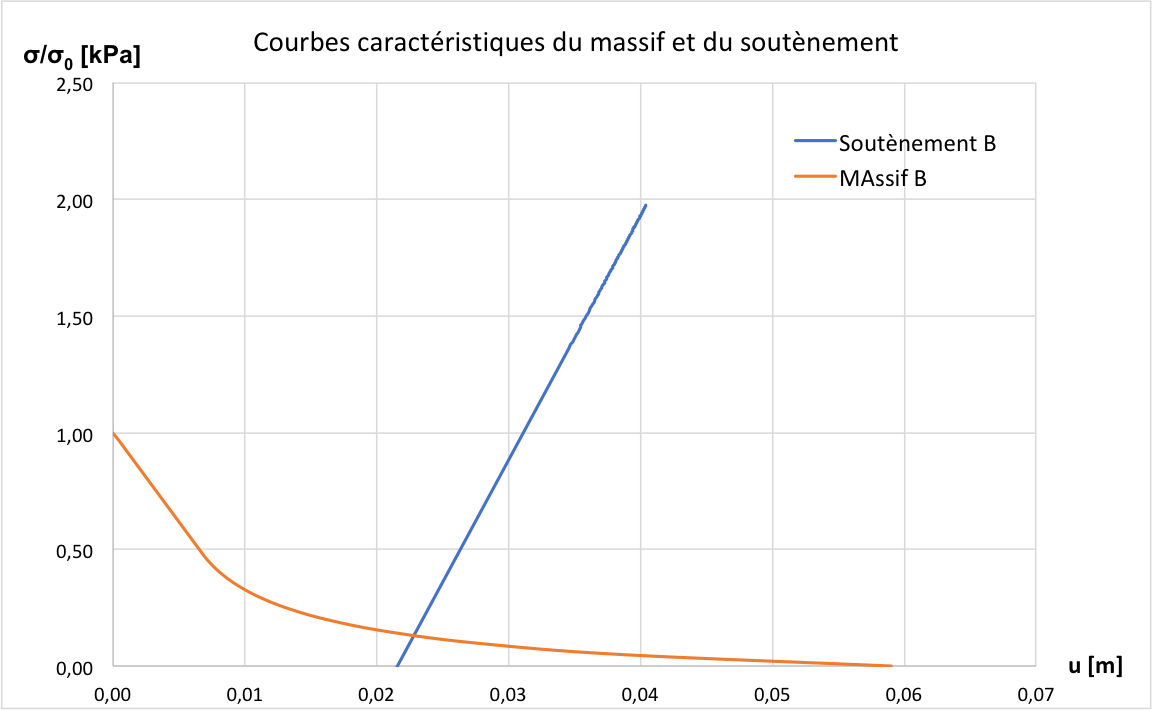
\includegraphics[width=10cm]{dimB.png}
\end{figure}
    \[d=3\text{m et }e=5\text{cm}\] 
\end{frame}






\section{Conclusion}

\begin{frame}{Conclusion}

\begin{itemize}
    \item Couche A la plus critique 
    \item Diminution du déplacement si 
    
    \begin{itemize}\scriptsize{
        \item[$\bullet$] l'épaisseur du soutènement augmente 
        \item[$\bullet$] la distance du soutènement par rapport au front de taille diminue
        \item[$\bullet$] le module de Young du béton augmente
        \item[$\bullet$] la cohésion augmente
        \item[$\bullet$] l'angle de frottement augmente}
    \end{itemize}
\end{itemize}
    
\end{frame}




\end{document}





